\section{Summarization and Discussion of Prior and Related Work}
\label{app:sec:prior_work}

\textbf{Prior Empirical Work} A growing body of recent work has investigated the phenomenon of iteratively training models on data generated by previous models, e.g., \citet{hataya2023will,martinez2023combining,shumailov2023curse, alemohammad2023self,martinez2023towards,bertrand2023stability,briesch2023large, dohmatob2024model, dohmatob2024tale} and (in a different context) \citet{taori2023data}.
\citet{hataya2023will} and \citet{martinez2023towards} conducted experiments replacing real training data with generated data at each iteration, assuming that the dataset size remains fixed over time. They found that this iterative retraining procedure can lead to model degradation if the proportion of synthetic data becomes too high. Similarly, \citet{shumailov2023curse} ran experiments with Gaussian mixture models, VAEs, and language models in which the total number of samples per iteration was held constant, and the samples always originated with the previous model rather than aggregating over time. Building on this work, \citet{alemohammad2023self} considered three treatments of data: fully replacing real data with synthetic data, augmenting a fixed real dataset with additional synthetic data, and mixing new real data with synthetic data at each iteration. In almost all of their experiments, they drew a fixed size dataset from the most recent model at each iteration, without accumulating data. \citet{bertrand2023stability} also assumed that dataset size and mixing proportions are constant over time in their theoretical stability analysis and empirical validation. %

\paragraph{Prior Theoretical Work} Over the last few years, there has been significant research effort contributing to our theoretical understanding of model behavior when synthetic data are integrated into training. The most closely related works to ours are \citet{dohmatob2024model} and \citet{dohmatob2024tale}; of course, the inspiration for the linear regression model studied in this paper directly comes from \citet{dohmatob2024model}. \citet{dohmatob2024model} performs an in-depth analysis of high dimensional linear and ridge regression when the training data used per iteration are generated from the previous iteration's fitted model. They are able to conclude that the test error grows linearly with the iteration count in their setup, as well as derive more interesting and more nuanced results using random matrix theory. They also discuss how to mitigate model collapse through optimal regularization both when the training data are noise-free and noisy versions of the previous model's synthetic outputs. A related noise-free setup was studied by \citet{mobahi2020self} in the case of self-distillation. Although \cite{mobahi2020self} considers a more general setup with ridge regression as a special case, they use \textit{noiseless} predictions from the previous model as the training data for the next model, and show that eventually, the predictions shrink to zero. Through this, they highlight that self-distillation induces regularization in the function space, which initially is beneficial for reducing over-fitting, but eventually over-regularization causes underfitting and hence performance decay. \cite{dohmatob2024tale} go beyond the linear model to study model collapse -- they study the tails of LLM outputs vs. real data and provide scaling laws that clearly identify regimes of model degradation when synthetic data misses \textit{tails} present in real data. They identify an interesting \textit{phase transition} in the test error scaling law depending on the size of the real dataset size in comparison to (a functional of) the chopped-off tail, and conclude that enough real data is able to mitigate model collapse. All these works consider the scenario where the amount of training data available per iteration is fixed (and does not grow with the iteration count), and it is certainly possible that with larger amount of synthetic data (from prediction by the previous model), several of these scalings would improve significantly. For example, in Equation (12) of \cite{dohmatob2024tale}, one obtains the linear scaling (with iteration count) of test error simply because the amount of synthetic data generated per iteration is the same. If one generated synthetic data with size proportional to the iteration count, then at iteration $n$, the scaling would, instead of $n$, be like $n^{1-c}/(1-c)$ for $c<1$. When one does not increase the dataset size, \cite{dohmatob2024tale} points out that increasing the proportion of real data would help one to avoid model collapse altogether. However, even if one \textit{did} increase the amount of synthetic data with iteration count, Theorem 3.2 coupled with Corollary 3.3 in \cite{dohmatob2024tale} would tell us that the \textit{amount} of real data was all that mattered -- if the amount of real data is large, we overcome model collapse. If one only had synthetic data (and no real data), no matter how large, it would be impossible to regain the original real-data scaling laws.
The scenario we study is highly inspired by these pioneering works, but still, in our view, different. We consider the case when we keep \textit{augmenting} synthetic data (generated by the previous model trained on all the previous data so far) as iterations progress, much akin to how -- in our view -- the internet evolves. We observe that we can avoid model collapse in this setting. The analysis of previous models in our case is more involved, since the data used for training at iteration $n$ is not homogeneous -- different models from the past impart different statistical aspects to different parts of the training data. We also note a related augmentation model studied by \cite{jain2024scaling} -- they perform risk minimization augmenting real data with synthetic data available from a potentially different independent source. One of their messages is that augmentation of (even) pure noise can be looked upon as adding a ridge penalty and hence, in certain cases, can improve test error. Their setup, however, is different from ours, since the synthetic data in their setup is not obtained by a learning algorithm employed on the real data, and the process is not iterative. However, morally, each iteration of ours involves risk minimization on data statistically composed of an equal mixture of data generated from the previous models, and hence each iteration of ours can be mapped to the general framework developed in \cite{jain2024scaling}, although the dependencies among the various models trained in our setup introduce theoretical complications that do not seem to be too easily addressed by the theory developed in \cite{jain2024scaling}. Shortly after v1 of our manuscript was uploaded to ArXiv, two other manuscripts appeared, dealing with the theoretical aspects in a setting similar to ours. Theorem 1 of \cite{marchi2024heat} obtains the same square summability scaling of the variance as us. \cite{seddik2024bad} studies collapse in language models in both purely synthetic and partly synthetic regimes and obtains deviation bounds as model iterations progress.

\begin{figure}[b!]
    \centering
    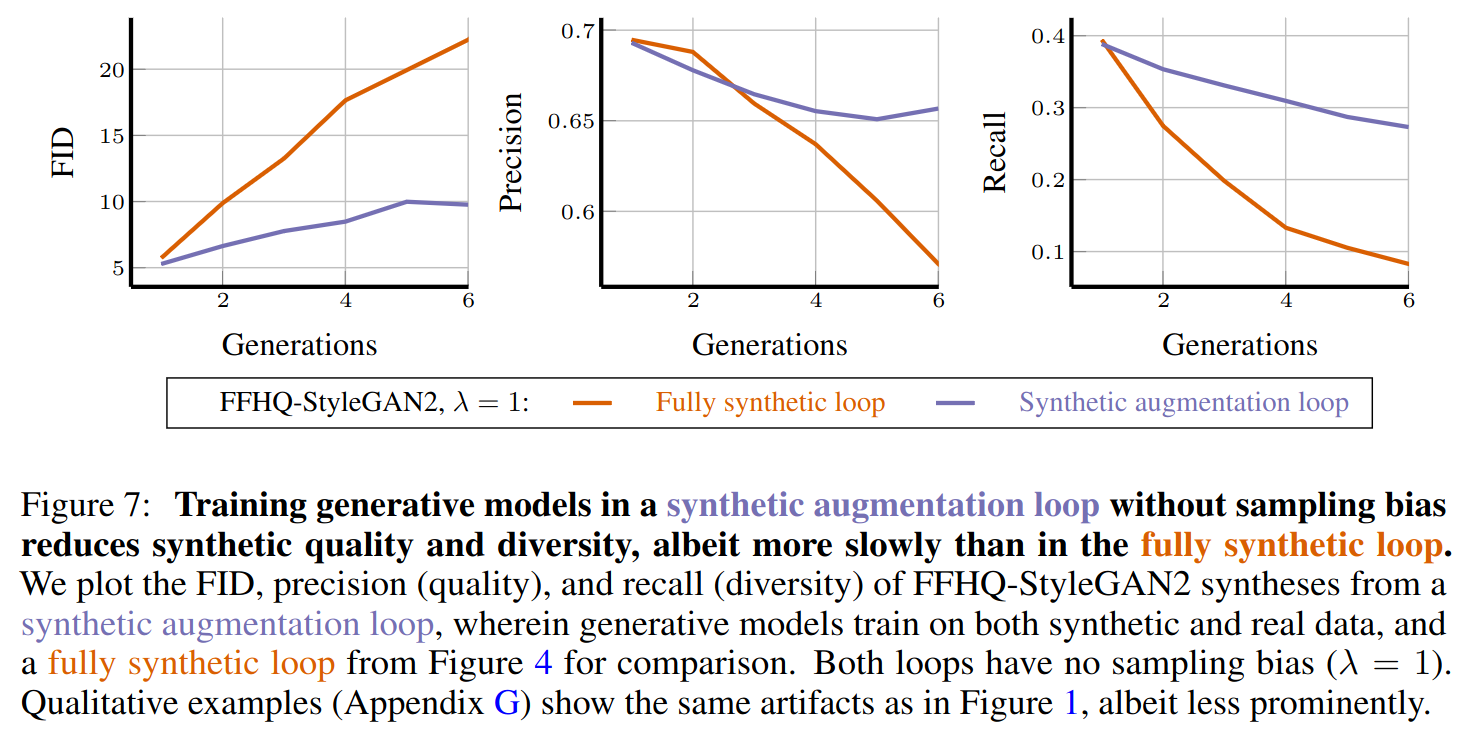
\includegraphics[trim={0 10cm 0 0},clip,width=\textwidth]{figures/appendix/alemohammad2023selfconsuming_fig7.png}
    \caption{\textbf{Clarification of Data Accumulation in \citet{alemohammad2023self}}. Figure 7 from \citet{alemohammad2023self} (above) shows that linearly accumulating data (``Synthetic augmentation loop") causes poor behavior to plateau with the number of model-fitting iterations. \citet{alemohammad2023self} write, ``Our experiments [...] support our main conclusion [that] fixed real training data only delays the inevitable degradation of the quality or diversity of the generative models over generations." We believe is that our evidence and their evidence is more consistent with the conclusion that accumulating data \textit{avoids} model collapse and does not merely delay it.}
    \label{app:fig:responding_to_alemohammad2023selfconsuming}
\end{figure}


\paragraph{Considering Accumulating Data} The two papers we found that partially considered accumulating data are \cite{martinez2023combining} and \cite{alemohammad2023self}. \cite{alemohammad2023self} did so in one-half of one experiment: StyleGAN2 trained on FliqrFaces 128$\times$128 (App. Fig. \ref{app:fig:responding_to_alemohammad2023selfconsuming}). The authors concluded that accumulating data does not avoid model collapse, but merely slows it down. However, we believe that a closer examination of their results (App. Fig. \ref{app:fig:responding_to_alemohammad2023selfconsuming}) reveals that accumulating data causes the test error to plateau to a relatively low error with increasing numbers of model-fitting iterations. This result would support our conclusion that accumulating data avoids model collapse and does not merely delay it. The results from \citet{martinez2023combining} are harder to evaluate; 
model collapse only seems to occur when the amount of synthetic data added per model-fitting iteration is 2$\times$ the total amount of accumulated data, and the subsequent work by the authors switched from accumulating data to replacing data \citep{martinez2023towards}. We think understanding what conditions and why these discrepancies exist is an interesting future direction.

\paragraph{Avoiding Model Collapse} Several papers present methods for avoiding or slowing model collapse. \citet{bertrand2023stability} shows in the replacing data setting that model collapse will not occur if the initial generative models approximate the data distribution well enough and the proportion of real data is sufficiently large with respect to the synthetic data.
\citet{dohmatob2024tale} similarly demonstrates that in the replacing data setting, carefully selecting real data to mix with synthetic data can avoid model collapse. Other solutions may also be possible in various models and under various assumptions. To our knowledge, no paper has claimed an ``optimal" strategy to avoid model collapse, and neither has ours.


\clearpage
\section{Proofs of Mathematical Results}
\label{app:sec:proofs}

We point out a lemma useful to prove Theorem \ref{thm:warmup_ridgeless_isotropic}.
\begin{lemma}
Let $T$ and $d$ be positive integers with $T \geq d + 2$, and let $X \in \mathbb{R}^{T \times d}$ be a random matrix with i.i.d. rows from $\mathcal{N}(0, \Sigma)$ with $\Sigma$ positive definite. Then, $X$ has full rank a.s. Moreover, it holds that:
\begin{equation}
\mathbb{E}_X[(X^\top X)^{-1}] = \frac{1}{T - d - 1} \Sigma^{-1}.
\end{equation}
\label{lemma:tr_inv_cov_eq_prefactor_inv_cov}
\end{lemma}

\begin{proof}
    See \citet{dohmatob2024model}.
\end{proof}

Assuming Lemma \ref{lemma:tr_inv_cov_eq_prefactor_inv_cov} and Theorem \ref{theorem:ridgeless_fitted_linear_parameters}, we present the proof of Theorem \ref{thm:warmup_ridgeless_isotropic}.

\begin{proof}[Proof of Theorem \ref{thm:warmup_ridgeless_isotropic}]
From Theorem \ref{theorem:ridgeless_fitted_linear_parameters}, we have:
\begin{equation}
\hat{w}_n = w^* + (X^\top X)^{-1} X^\top \left(\sum_{i=1}^n \frac{E_i}{i}\right)
\end{equation}
where $w^*$ is the true parameter, $X$ is the original data matrix, and $E_i$ are the noise terms at each iteration, with $E_i \sim \mathcal{N}(0, \sigma^2 I_T)$. The test error is given by:
\begin{equation}
E_{\text{test}}(\hat{w}_n) = \mathbb{E}[||\hat{w}_n - w^*||_{\Sigma}^2]
\end{equation}where the expectation is taken over all random quantities involved.

Substituting $\hat{w}_n$ into the test error expression and using the fact that $\Sigma \defeq I_d$, we get:
\begin{align*}
E_{\text{test}}(\hat{w}_n) &= \mathbb{E}\left[\left(\sum_{i=1}^n \frac{E_i}{i}\right)^\top X(X^\top X)^{-2} X^\top \left(\sum_{i=1}^n \frac{E_i}{i}\right)\right] \\
&= \mathbb{E}\left[\sum_{i=1}^n \frac{\sigma^2}{i^2} \text{tr}(X(X^\top X)^{-2} X^\top)\right] \\
&= \sum_{i=1}^n \frac{\sigma^2}{i^2} \mathbb{E}\left[\text{tr}((X^\top X)^{-1})\right]
\end{align*}

Using Lemma \ref{lemma:tr_inv_cov_eq_prefactor_inv_cov}, we have:
\begin{equation}
\mathbb{E}_{X}\left[\text{tr}((X^\top X)^{-1})\right] = \frac{d}{T-d-1}
\end{equation}

Therefore, the test error for ridgeless regression with isotropic features in the data accumulation setting is:
\begin{align*}
E_{\text{test}}(\hat{w}_n) &= \sum_{i=1}^n \frac{\sigma^2}{i^2} \cdot \frac{d}{T-d-1} < \frac{\sigma^2 d}{T-d-1} \left(\frac{\pi^2}{6}\right)
\end{align*}
as $\sum_{i=1}^n i^{-2} < \sum_{i=1}^\infty i^{-2} = \pi^2/6$.
\end{proof}

Finally, we prove Theorem \ref{theorem:ridgeless_fitted_linear_parameters}.

\begin{proof}[Proof of Theorem \ref{theorem:ridgeless_fitted_linear_parameters}]

We prove this theorem by induction.

\textbf{Base case:} For $n=1$, we have:
\begin{align*}
\hat{w}_1 &= \tilde{X}_1^{\dagger} \tilde{Y}_1 = (X^\top X)^{-1} X^\top (Xw^* + E_1) = w^* + (X^\top X)^{-1} X^\top E_1
\end{align*}
which satisfies the lemma.

\textbf{Inductive step:} Assume that for some $n \geq 1$, we have:

\begin{equation*}
\hat{w}_n = w^* + (X^\top X)^{-1} X^\top \left(\sum_{i=1}^n \frac{E_i}{i}\right)
\end{equation*}

Now, consider $\hat{w}_{n+1}$:
\begin{align*}
\hat{w}_{n+1} &= \tilde{X}_{n+1}^{\dagger} \tilde{Y}_{n+1} \\
&= (\tilde{X}_{n+1}^\top \tilde{X}_{n+1})^{-1} \tilde{X}_{n+1}^\top \tilde{Y}_{n+1} \\
&= \frac{1}{n+1}(X^\top X)^{-1} \sum_{i=1}^{n+1} X^\top \hat{Y}_i
\end{align*}

Recalling that $\hat{Y}_i$:
\begin{align*}
\hat{Y}_i = \begin{cases}
X w^* + E_1, & i = 1 \\
X \hat{w}_{i-1} + E_i, & 2 \leq i \leq n+1
\end{cases}
\end{align*}

Substituting this back into the expression for $\hat{w}_{n+1}$:
\begin{align*}
\hat{w}_{n+1} &= \frac{1}{n+1}(X^\top X)^{-1} \left(X^\top (X w^* + E_1) + \sum_{i=2}^{n+1} X^\top (X\hat{w}_{i-1} + E_i)\right) \\
&= \frac{1}{n+1}(X^\top X)^{-1} \left(X^\top Xw^* + X^\top E_1 + \sum_{i=2}^{n+1} (X^\top X\hat{w}_{i-1} + X^\top E_i)\right) \\
&= \frac{1}{n+1}(X^\top X)^{-1} \left(X^\top Xw^* + X^\top E_1 + \sum_{i=1}^{n} (X^\top X\hat{w}_i + X^\top E_{i+1})\right) \\
&= \frac{1}{n+1}(X^\top X)^{-1} \left(X^\top X w^* + \sum_{i=1}^{n} X^\top X\hat{w}_i + \sum_{i=1}^{n+1} X^\top E_i\right)
\end{align*}

Now, using the induction hypothesis:
\begin{align*}
\hat{w}_{n+1} &= \frac{1}{n+1}(X^\top X)^{-1} \left(X^\top Xw^* + \sum_{i=1}^{n} X^\top X\left(w^* + (X^\top X)^{-1} X^\top \sum_{j=1}^i \frac{E_j}{j}\right) + \sum_{i=1}^{n+1} X^\top E_i\right) \\
&= \frac{1}{n+1}(X^\top X)^{-1} \left((n+1)X^\top Xw^* + \sum_{i=1}^{n} X^\top X(X^\top X)^{-1} X^\top \sum_{j=1}^i \frac{E_j}{j} + \sum_{i=1}^{n+1} X^\top E_i\right) \\
&= w^* + \frac{1}{n+1}(X^\top X)^{-1} \left(\sum_{i=1}^{n} X^\top \sum_{j=1}^i \frac{E_j}{j} + \sum_{i=1}^{n+1} X^\top E_i\right) \\
&= w^* + \frac{1}{n+1}(X^\top X)^{-1} X^\top \left(\sum_{i=1}^{n} \sum_{j=1}^i \frac{E_j}{j} + \sum_{i=1}^{n+1} E_i\right)
\end{align*}

Now, we need to simplify the term $\sum_{i=1}^{n} \sum_{j=1}^i \frac{E_j}{j} + \sum_{i=1}^{n+1} E_i$. We can do this by counting the number of times each $E_i$ appears in the double sum: $E_1$ appears $n$ times in the double sum and once in the single sum, so its coefficient is $\frac{n+1}{1}$. $E_2$ appears $n-1$ times in the double sum and once in the single sum, so its coefficient is $\frac{n}{2}$. This continues along till we reach $E_n$, which appears once in the double sum and once in the single sum, so its coefficient is $\frac{2}{n}$. $E_{n+1}$ appears only once in the single sum, so its coefficient is $\frac{1}{n+1}$. Therefore,
\begin{align*}
\sum_{i=1}^{n} \sum_{j=1}^i \frac{E_j}{j} + \sum_{i=1}^{n+1} E_i &= \sum_{i=1}^{n+1} \frac{n+2-i}{i} E_i = (n+1) \sum_{i=1}^{n+1} \frac{E_i}{i}
\end{align*}

Substituting this back into the expression for $\hat{w}_{n+1}$:
\begin{align*}
\hat{w}_{n+1} &= w^* + \frac{1}{n+1}(X^\top X)^{-1} X^\top \left((n+1) \sum_{i=1}^{n+1} \frac{E_i}{i}\right) \\
&= w^* + (X^\top X)^{-1} X^\top \sum_{i=1}^{n+1} \frac{E_i}{i}
\end{align*}



Therefore, by mathematical induction, the lemma holds for all $n \geq 1$.
\end{proof}





\clearpage
\section{Additional Details and Ablations on Language Model Experiments}
\label{app:sec:lm_ablations}
\subsection*{Implementation Details}
Model training was implemented using Huggingface Transformers~\citep{wolf2019huggingface}. Dataset generation was implemented using vllm~\citep{kwon2023efficient}.

\subsection*{Additional Plots}
In addition to Figure~\ref{fig:language_modeling_results_learning_curves} in the main text, Figures~\ref{app:fig:language_modeling_results_learning_curves_epochs_lin}-\ref{app:fig:language_modeling_results_learning_curves_steps_log} show learning curves in larger print, with x-axes showing either epochs or gradient steps, and with axes shown in linear-linear or log-log scale, respectively.



\begin{figure}
    \centering
    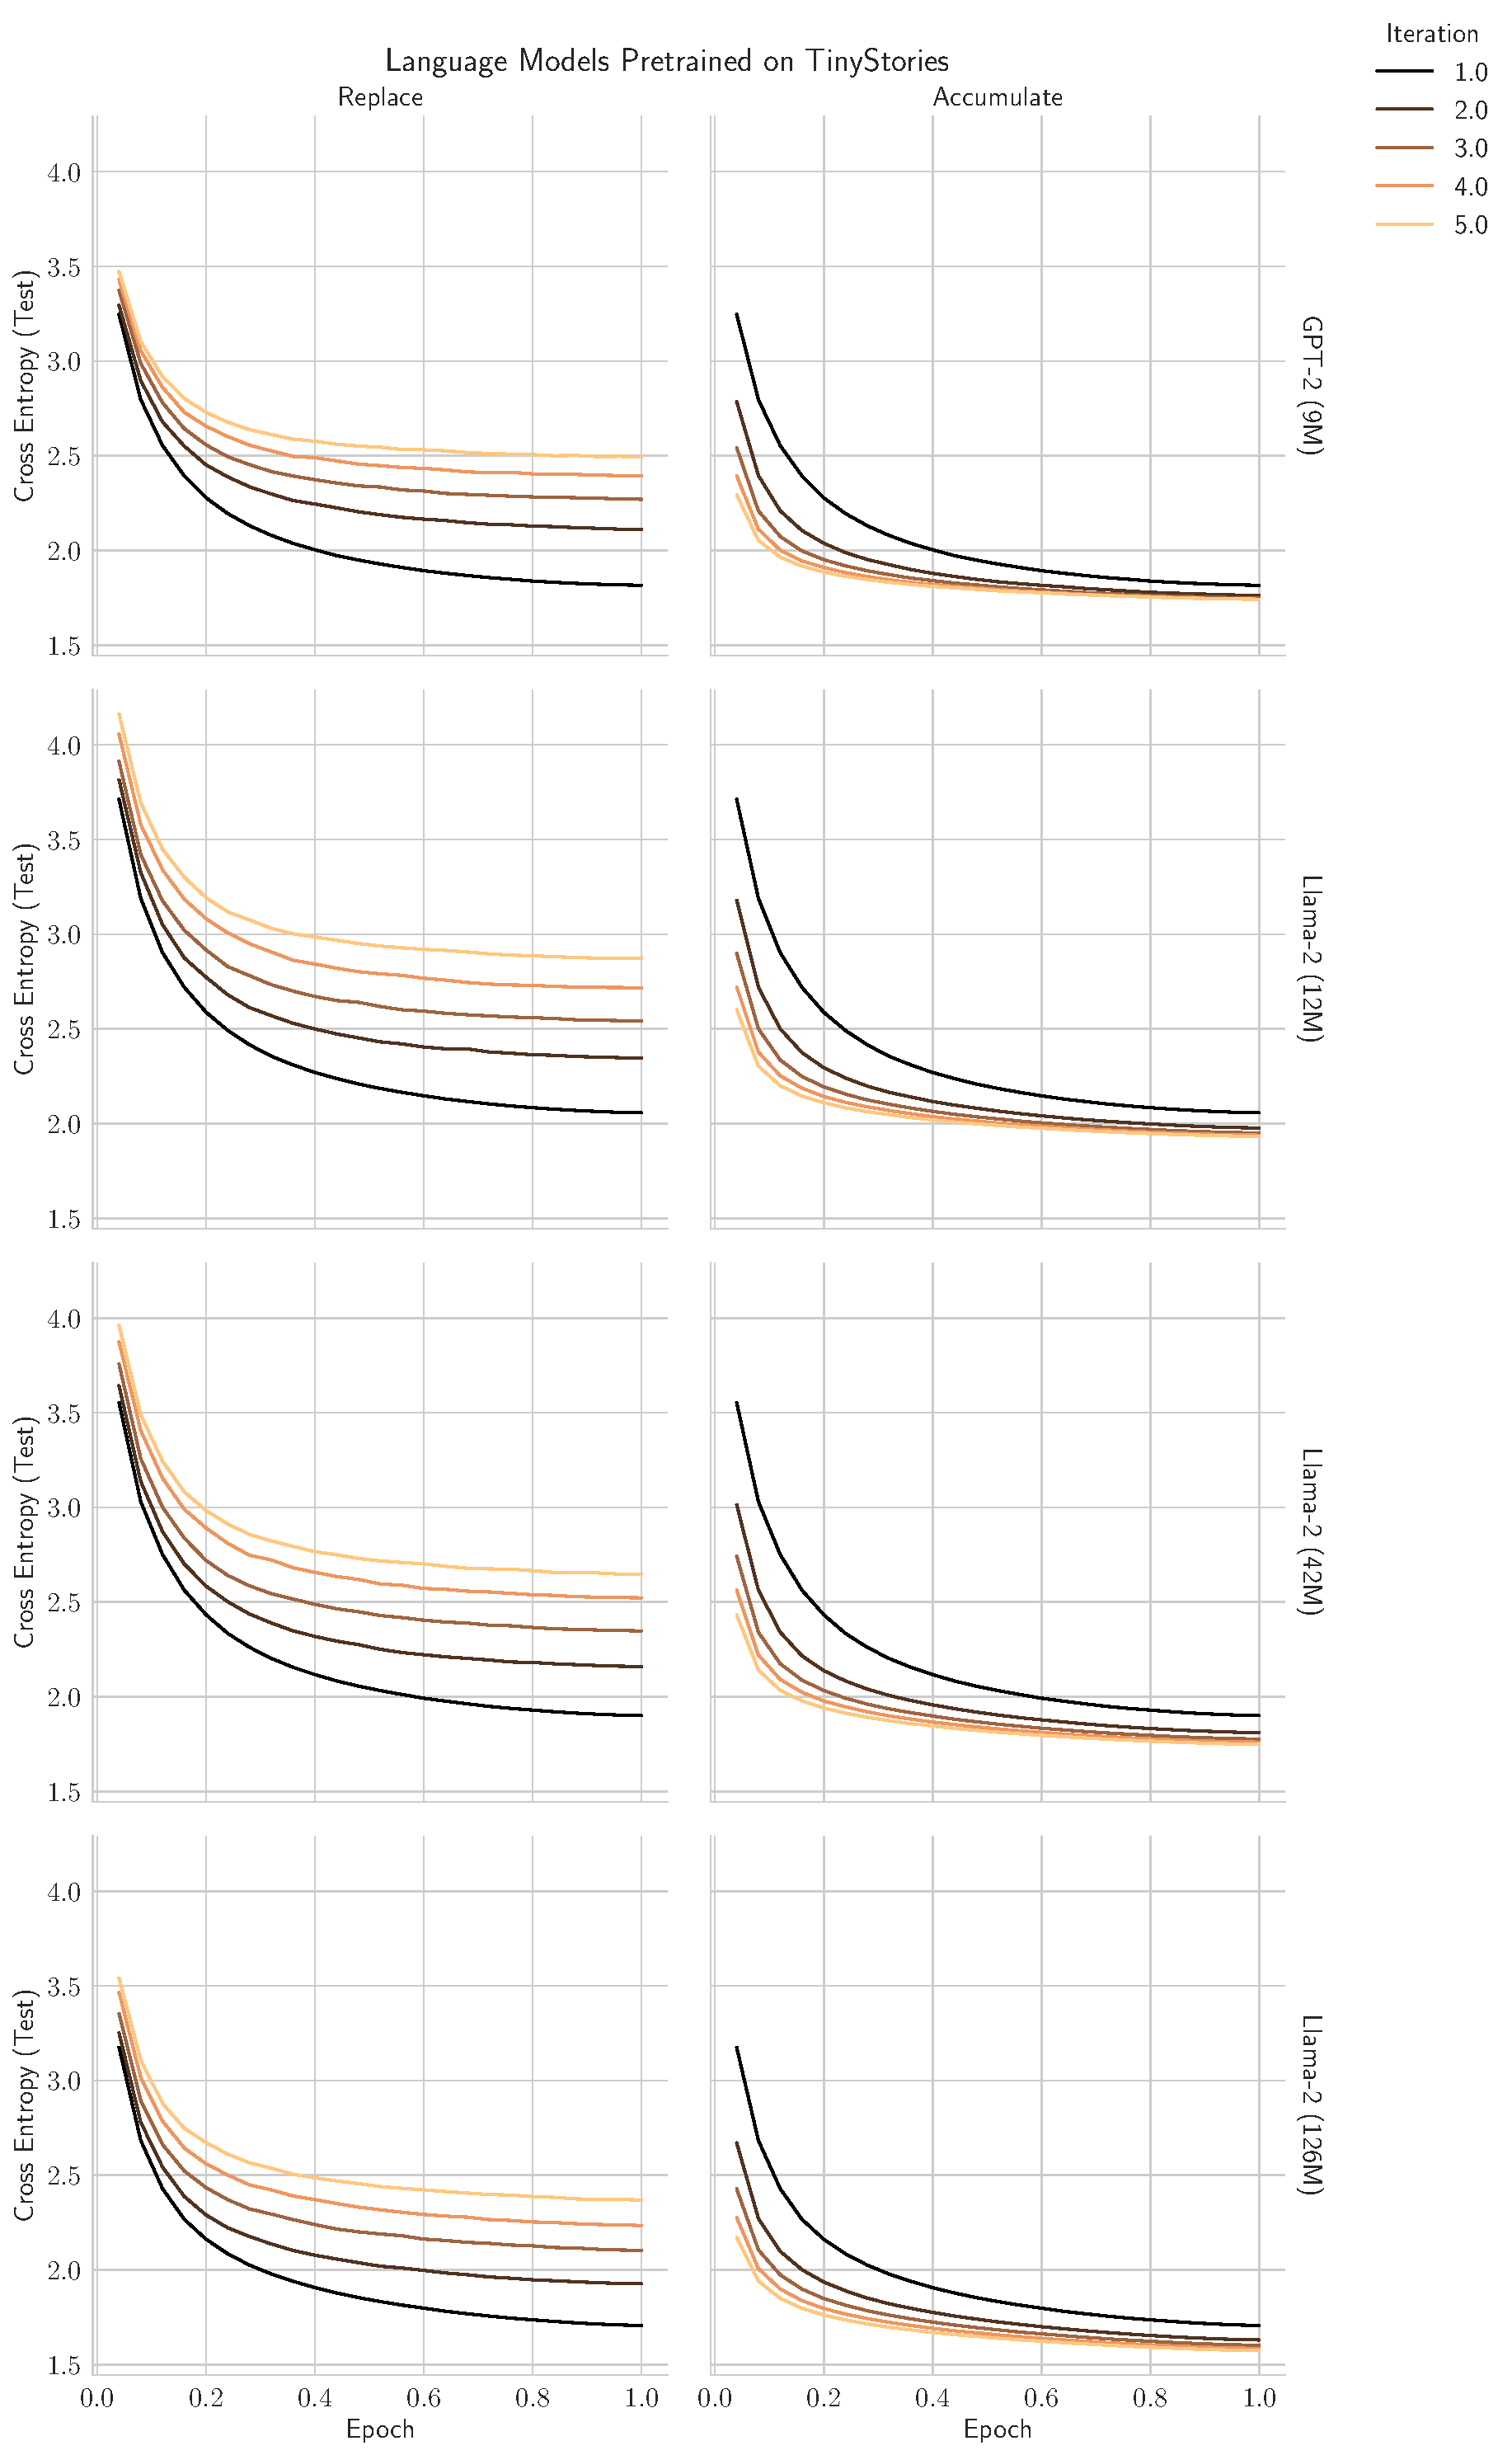
\includegraphics[width=0.9\textwidth]{figures/language_modeling/eval_loss_linear_vs_epoch_linear_flipped_20240403.pdf}
    \caption{\textbf{Data Accumulation Avoids Model Collapse in Language Modeling.} Learning curves for individual model-fitting iterations when repeatedly \textit{replacing} data (left), and when \textit{accumulating} data (right). Note: Epochs correspond to more gradient steps for accumulate than replace because the number of training data grows for accumulate.
    }
    \label{app:fig:language_modeling_results_learning_curves_epochs_lin}
\end{figure}


\begin{figure}
    \centering
    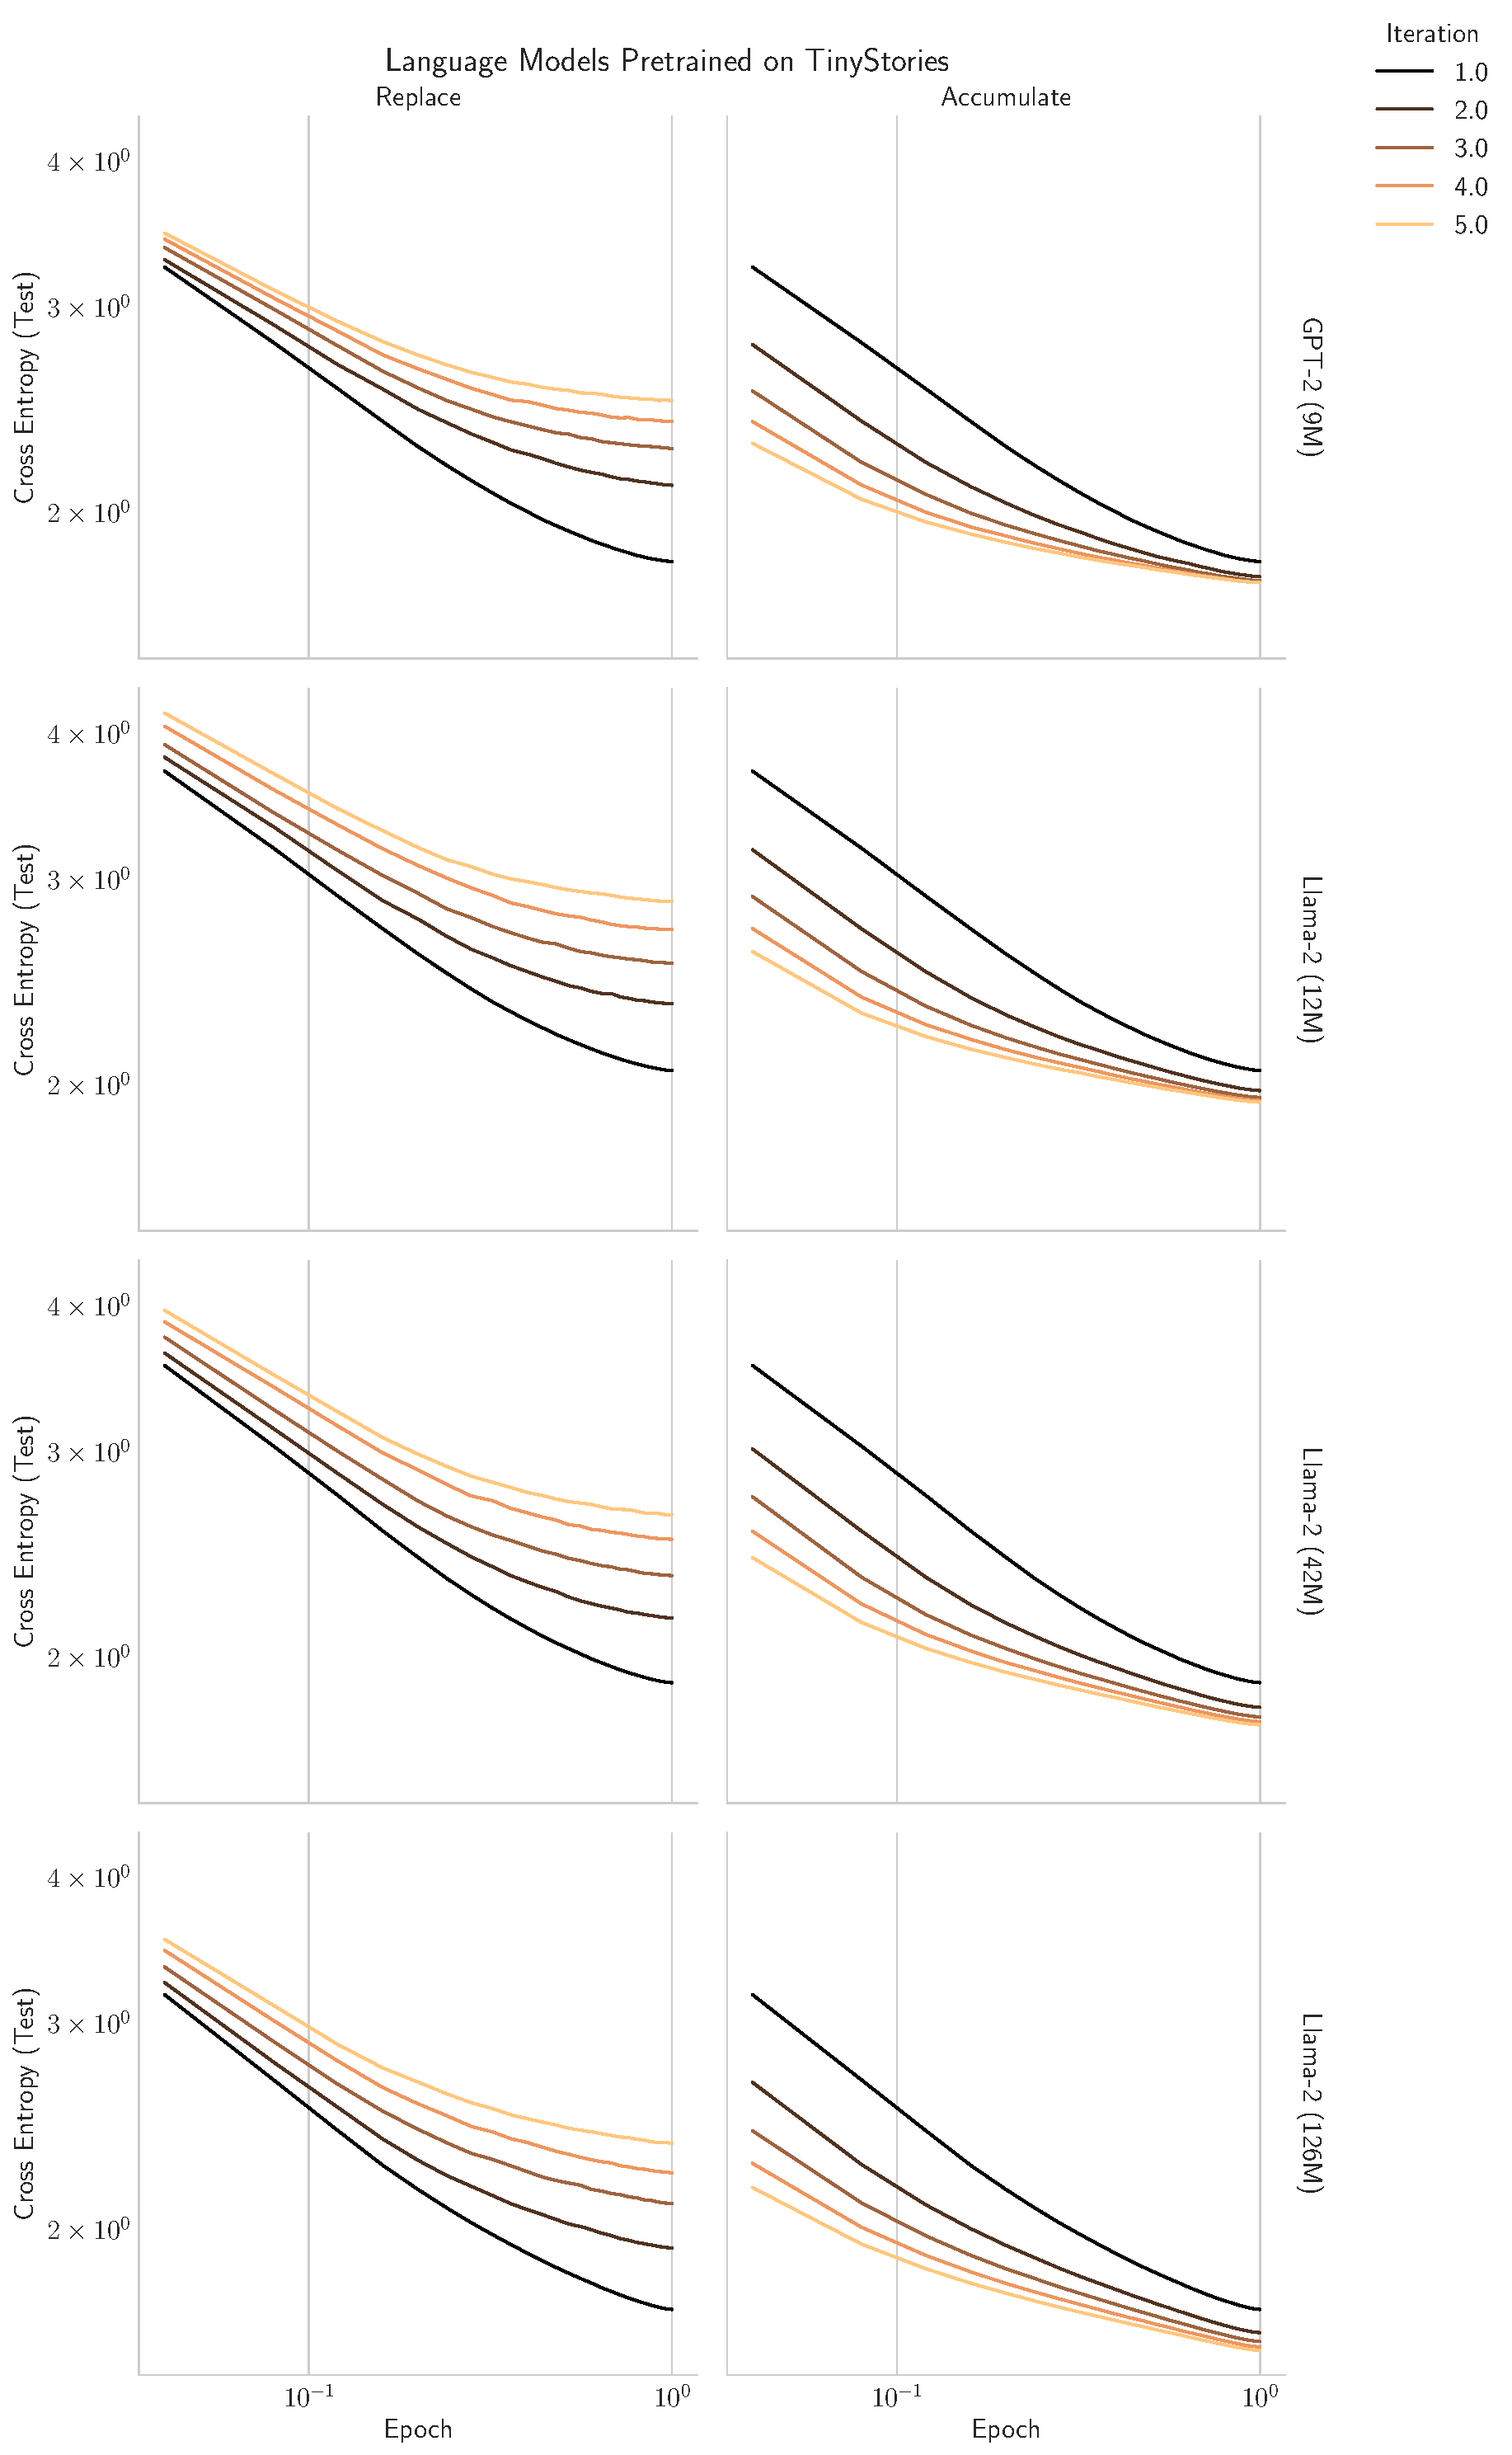
\includegraphics[width=0.9\textwidth]{figures/language_modeling/eval_loss_log_vs_epoch_linear_flipped_20240403.pdf}
    \caption{\textbf{Data Accumulation Avoids Model Collapse in Language Modeling.} Learning curves for individual model-fitting iterations when repeatedly \textit{replacing} data (left), and when \textit{accumulating} data (right), in log-log scale. Note: Epochs correspond to more gradient steps for accumulate than replace because the number of training data grows for accumulate.
    }
    \label{app:fig:language_modeling_results_learning_curves_epochs_log}
\end{figure}



\begin{figure}
    \centering
    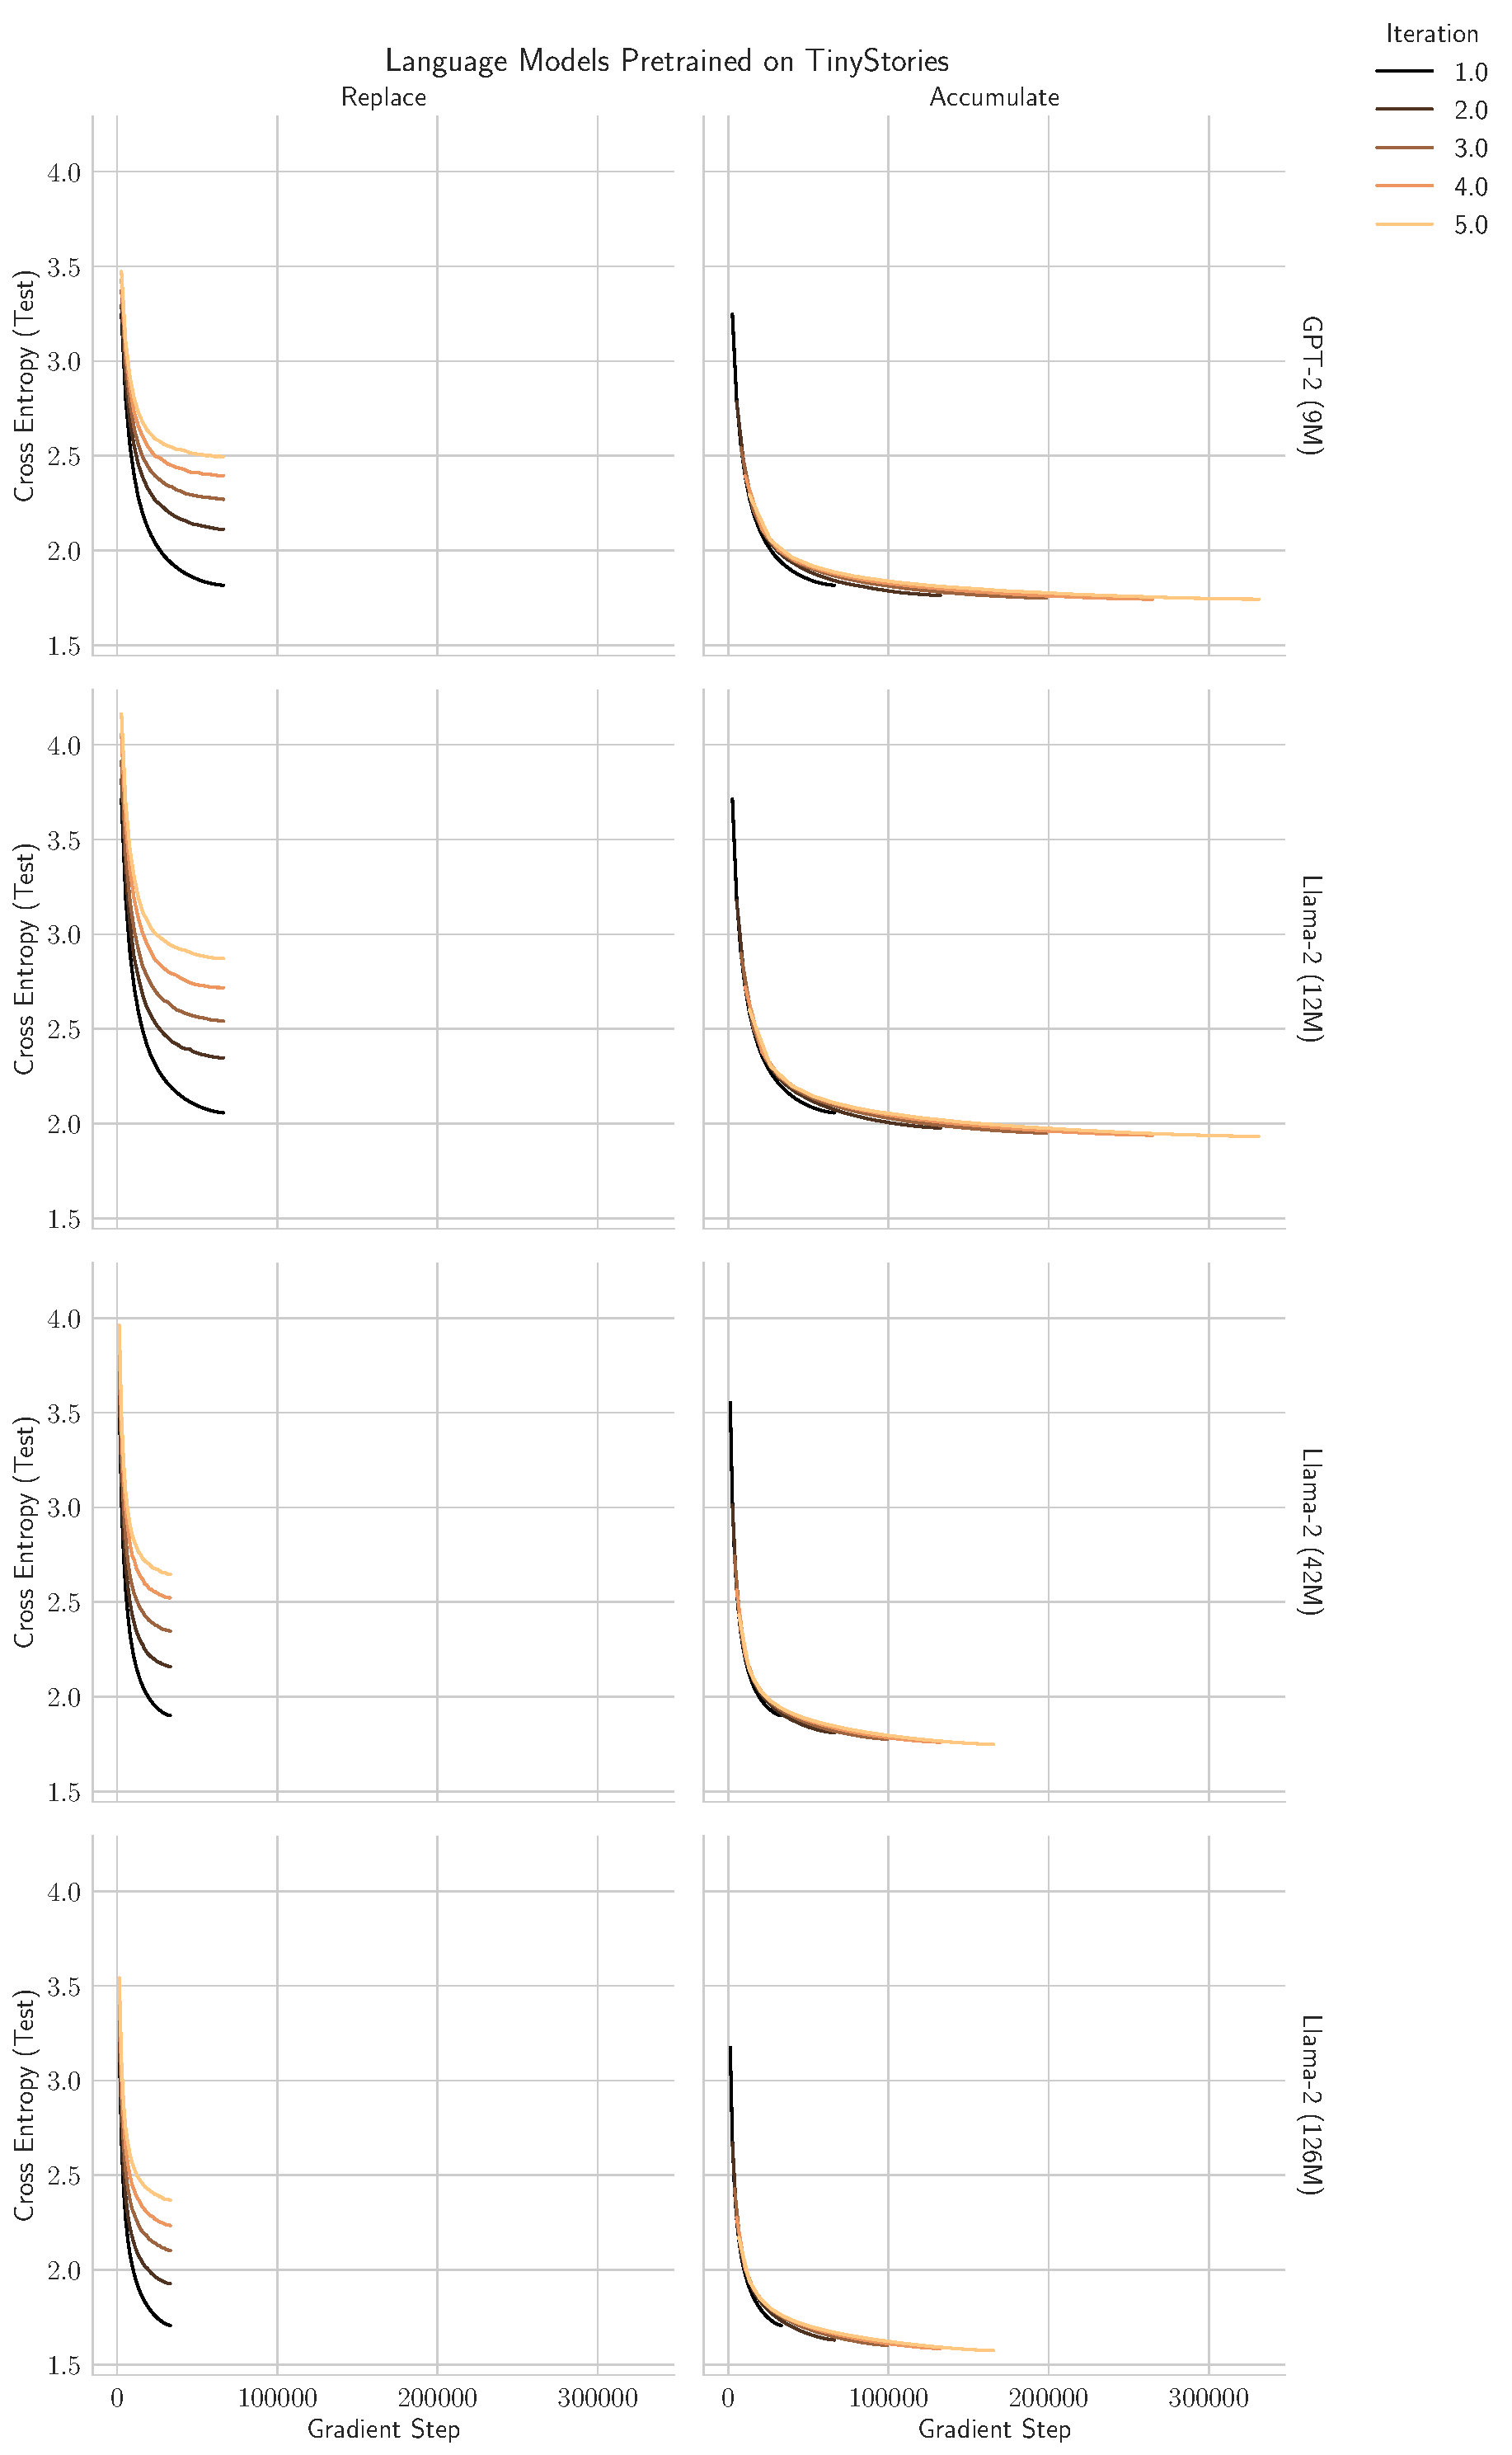
\includegraphics[width=0.9\textwidth]{figures/language_modeling/eval_loss_linear_vs_trainer_global_step_linear_flipped_20240403.pdf}
    \caption{\textbf{Data Accumulation Avoids Model Collapse in Language Modeling.} Learning curves for individual model-fitting iterations when repeatedly \textit{replacing} data (left), and when \textit{accumulating} data (right).
    }
    \label{app:fig:language_modeling_results_learning_curves_steps_lin}
\end{figure}


\begin{figure}
    \centering
    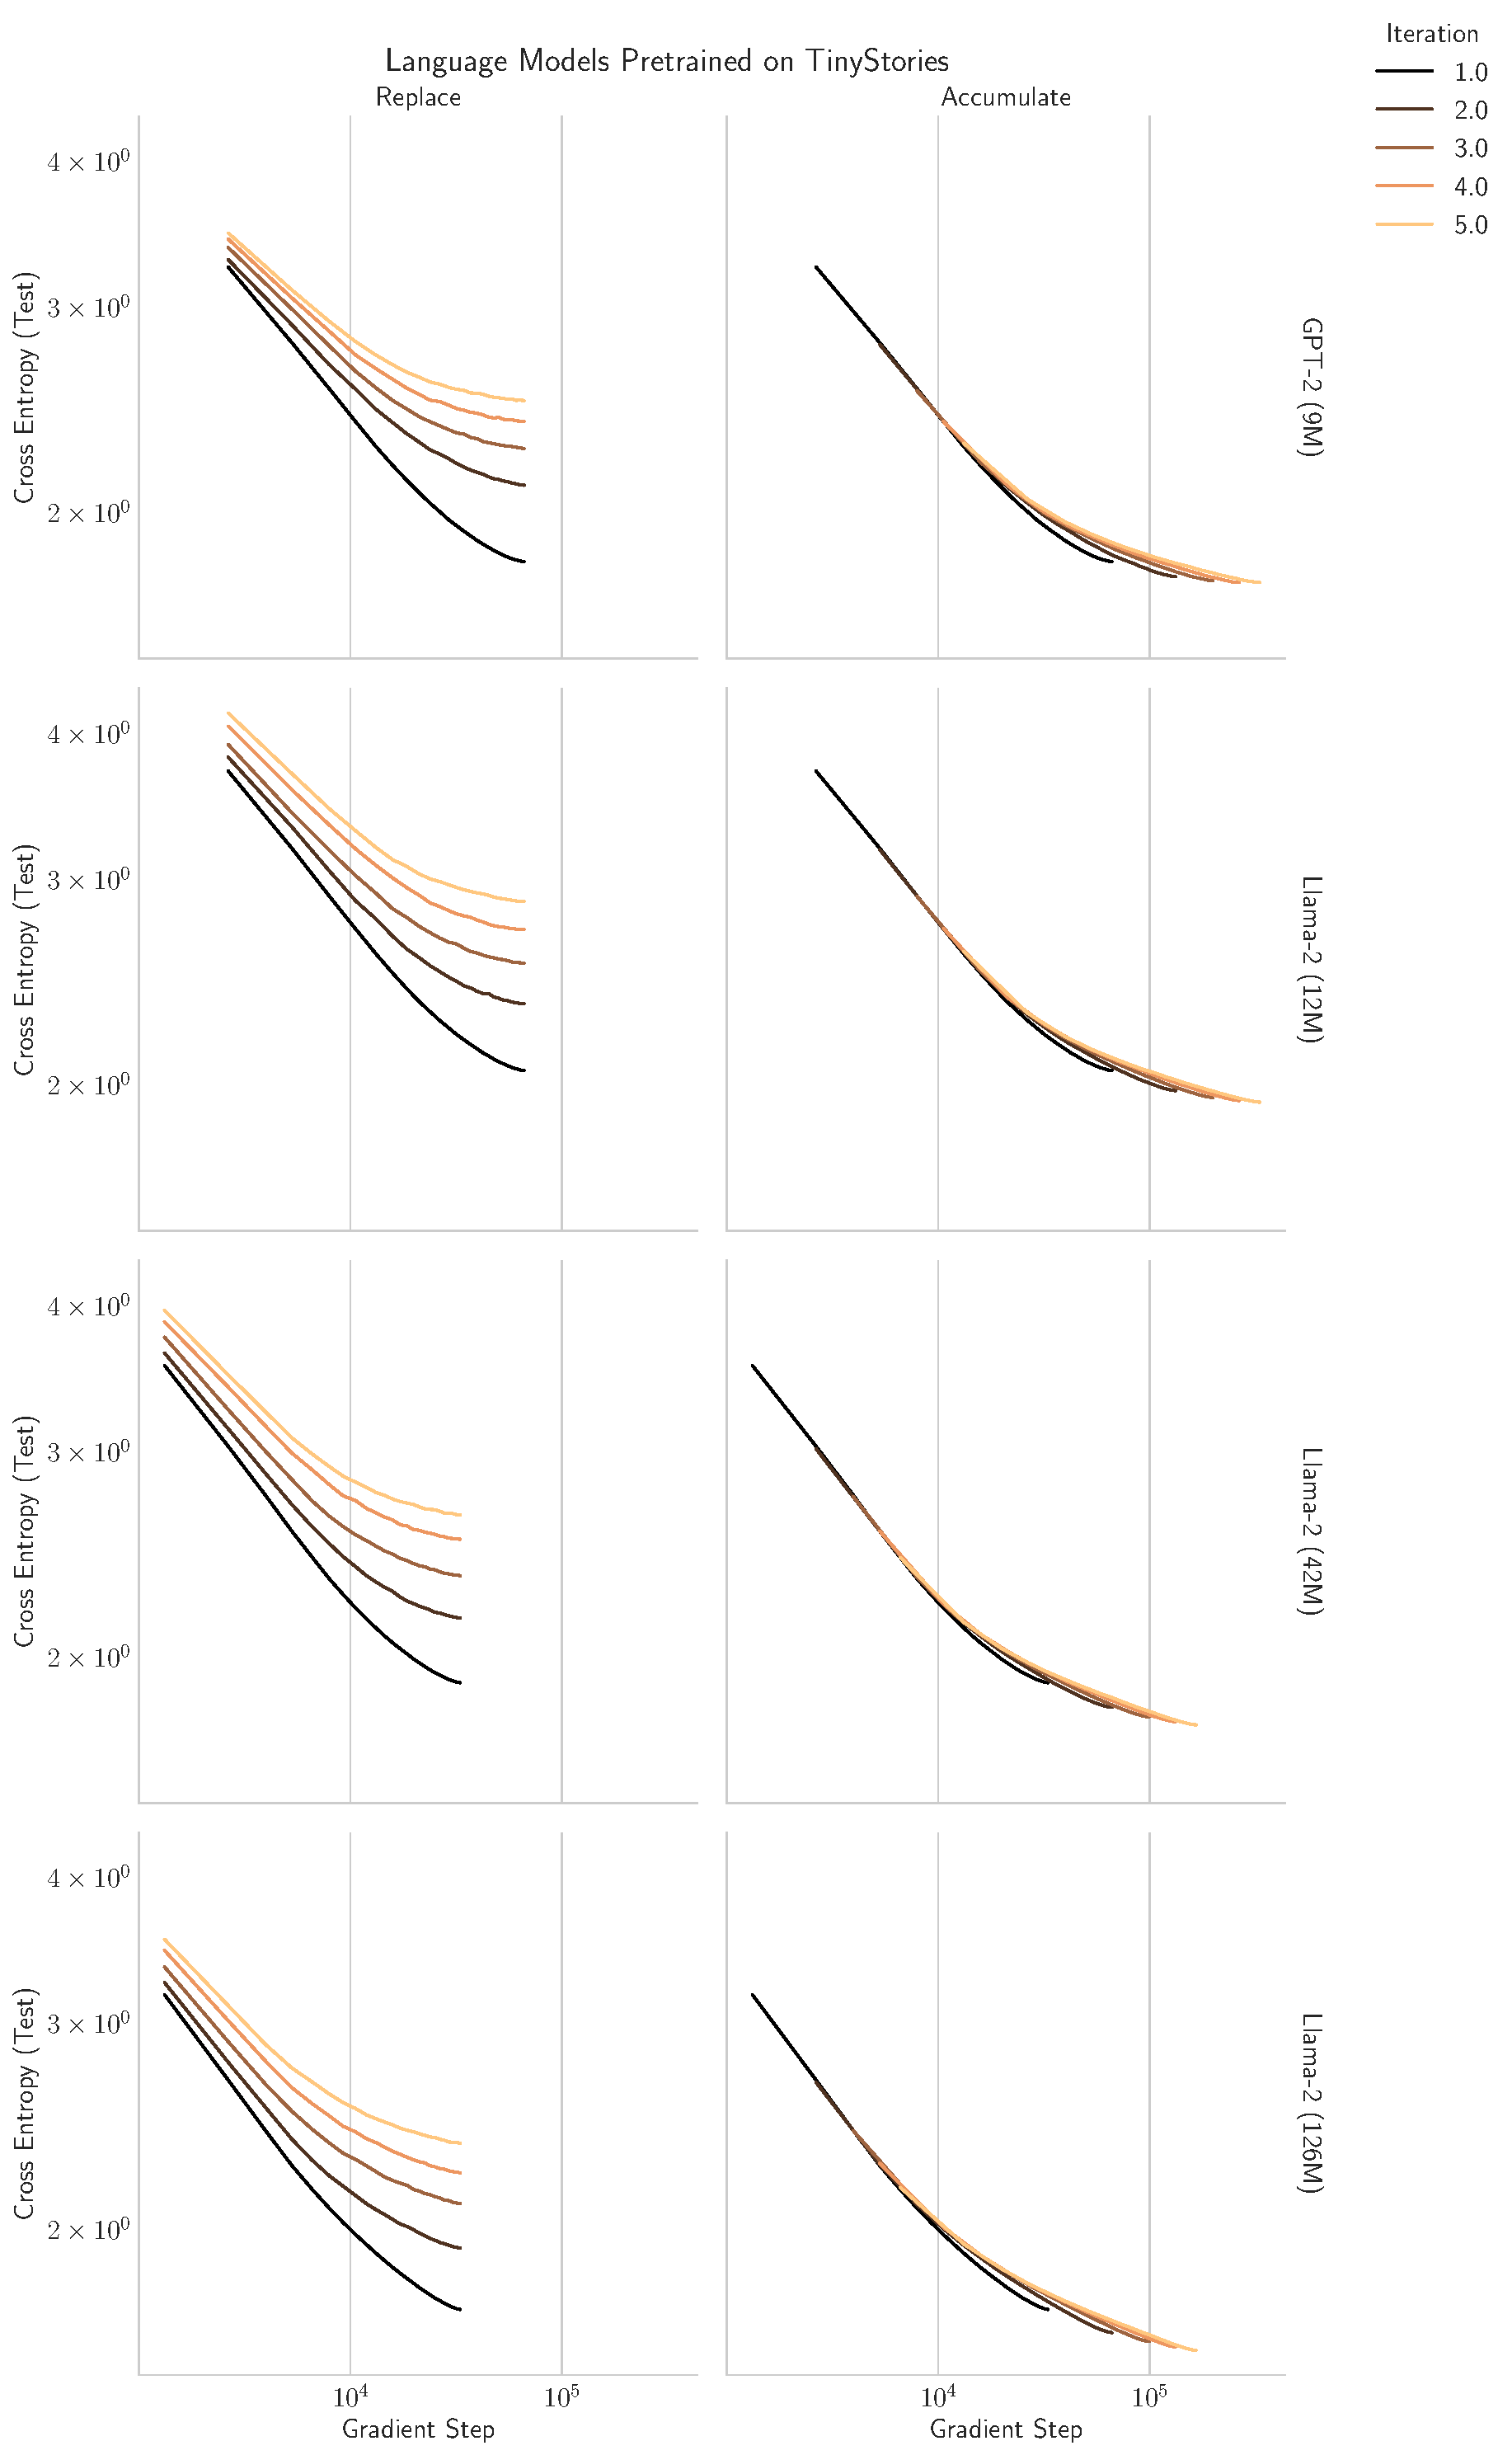
\includegraphics[width=0.9\textwidth]{figures/language_modeling/eval_loss_log_vs_trainer_global_step_linear_flipped_20240403.pdf}
    \caption{\textbf{Data Accumulation Avoids Model Collapse in Language Modeling.} Learning curves for individual model-fitting iterations when repeatedly \textit{replacing} data (left), and when \textit{accumulating} data (right), in log-log scale.
    }
    \label{app:fig:language_modeling_results_learning_curves_steps_log}
\end{figure}

\subsection*{Ablations}
In addition to the experiments shown in the main paper, we conducted several ablation studies.

\paragraph{Controlling for dataset size.} One possible concern is that when accumulating data, the train dataset size will grow at each model-fitting iteration, meaning subsequent models will be trained on more aggregate data than their counterparts in the replacement regime. To control for this, we run experiments controlling for this. In this ``replace-multiple'' regime, we create a fully synthetic dataset at the end of each model-fitting iteration, but grow the size of this dataset to match that of the accumulated data in the accumulation regime. Table~\ref{tab:lm_eval_loss} rightmost column shows that in this regime, evaluation loss still increases over model-fitting iterations.

\paragraph{Generation temperature.} Most of our language model experiments were run with sampling temperature $1.0$ during generation of new datasets. To ensure that this choice is not critical, we also run one experiment with temperature $0.3$, and see that this shows similar results (with even larger increases in validation loss in the replacement regime than temperature $1.0$), as shown in Table~\ref{tab:lm_eval_loss}, row 2, and Figure~\ref{fig:language_modeling_temp}.

\paragraph{Dataset size and training epochs.} We similarly vary the size of the initial (and subsequent) training datasets and number of training epochs, and see that this has no qualitative effect on the results (Table~\ref{tab:lm_eval_loss}, rows 3 \& 4 show training on 1/5th of the TinyStories dataset for 1 \& 3 epochs, respectively).

\paragraph{Model quality after first model-fitting iteration.} Finally, we control specifically for model (and thus synthetic dataset) quality after the first iteration, to rule out an undue influence of a ``bad'' first synthetic dataset on subsequent training. Figure~\ref{fig:language_modeling_firstiter} shows performance in subsequent iterations for different amounts of training in the first iteration, showing no qualitative differences.

\begin{table}[h!]
    \centering
    \begin{tabular}{c|c|c|c|c|c}
        Model & t=1 & t=4 (acc) & t=4 (repl) & t=10 (repl) & t=4 (*) \\
        \hline 
GPT-2 (9M) & 1.82 & 1.74 (-0.07) & 2.39 (+0.58) & 2.91 (+1.09) & 2.18 (+0.36) \\
GPT-2 (9M) (temp=0.3) & 1.82 & 1.75 (-0.06) & 5.82 (+4.00) & 9.85 (+8.04) & n/a \\
GPT-2 (9M) (small dataset) & 2.56 & 2.28 (-0.28) & 3.21 (+0.65) & 3.72 (+1.16) & 2.91 (+0.35) \\
ibid (+ 3 epochs) & 1.99 & 1.87 (-0.12) & 2.62 (+0.63) & n/a & n/a \\
Llama-2 (12M) & 2.06 & 1.94 (-0.12) & 2.72 (+0.66) & n/a & n/a \\
Llama-2 (42M) & 1.90 & 1.76 (-0.14) & 2.52 (+0.62) & n/a & n/a \\
Llama-2 (126M) & 1.71 & 1.59 (-0.12) & 2.23 (+0.53) & n/a & n/a \\
    \end{tabular}
    \caption{Evaluation cross-entropy loss for different models at model-fitting iterations 1, 4 and 10 for replacement and accumulation regimes. (*) indicates a replacement regime with growing dataset size to ablate for total train set size.}
    \label{tab:lm_eval_loss}
\end{table}



\begin{figure}
    \centering
    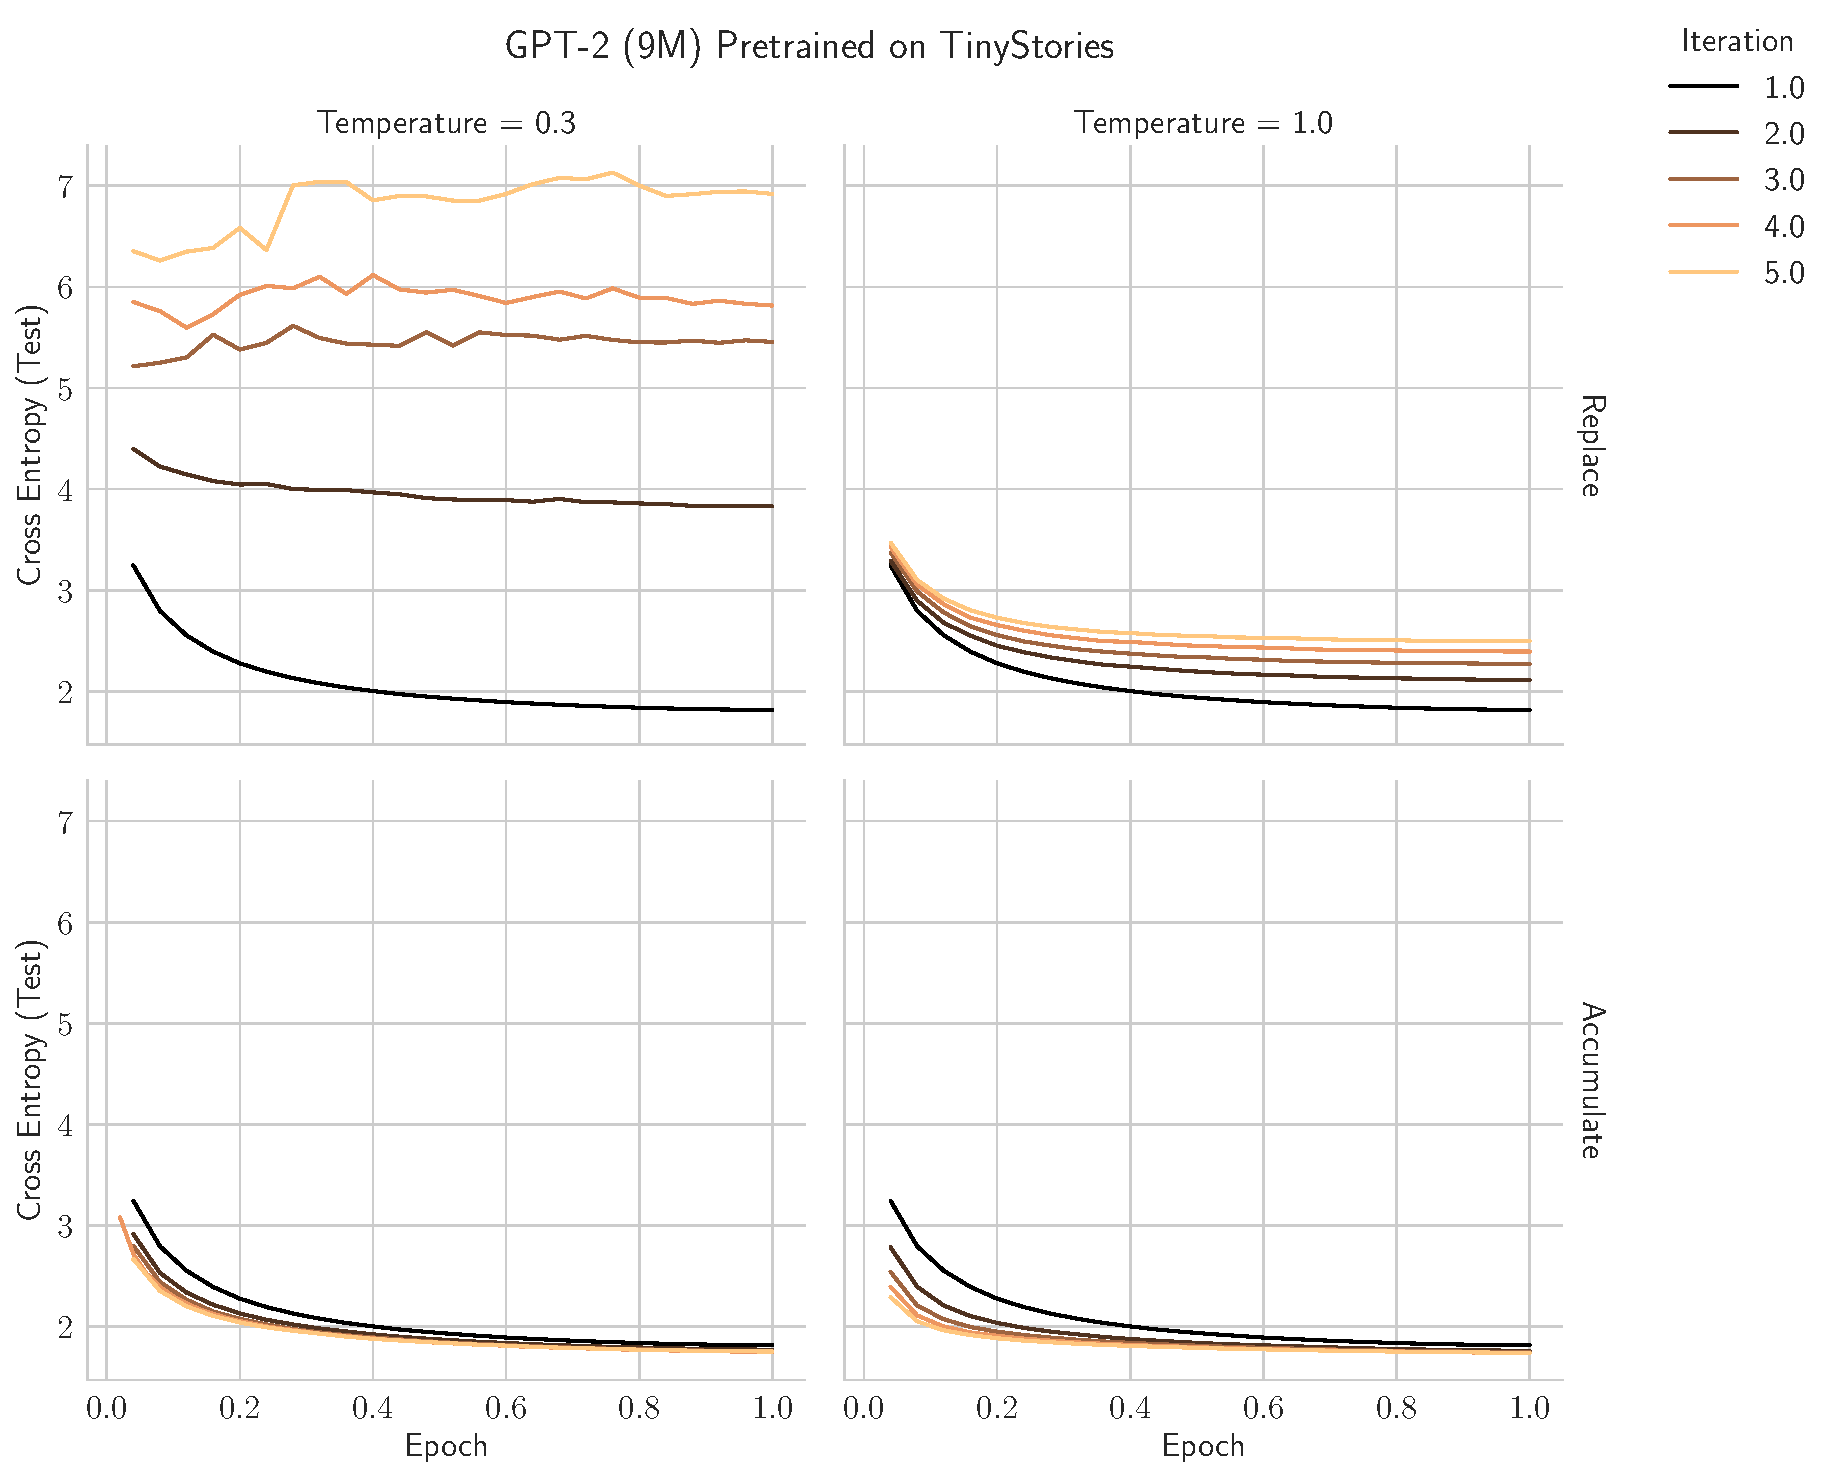
\includegraphics[width=0.7\textwidth]{figures/language_modeling/eval_loss_linear_vs_epoch_temperature_20240329_220900.pdf}
    \caption{Accumulating data shows stable behavior across different generation temperatures for a GPT-2 (9M) model, while replacing data does not.
    }
    \label{fig:language_modeling_temp}
\end{figure}




\begin{figure}
    \centering
    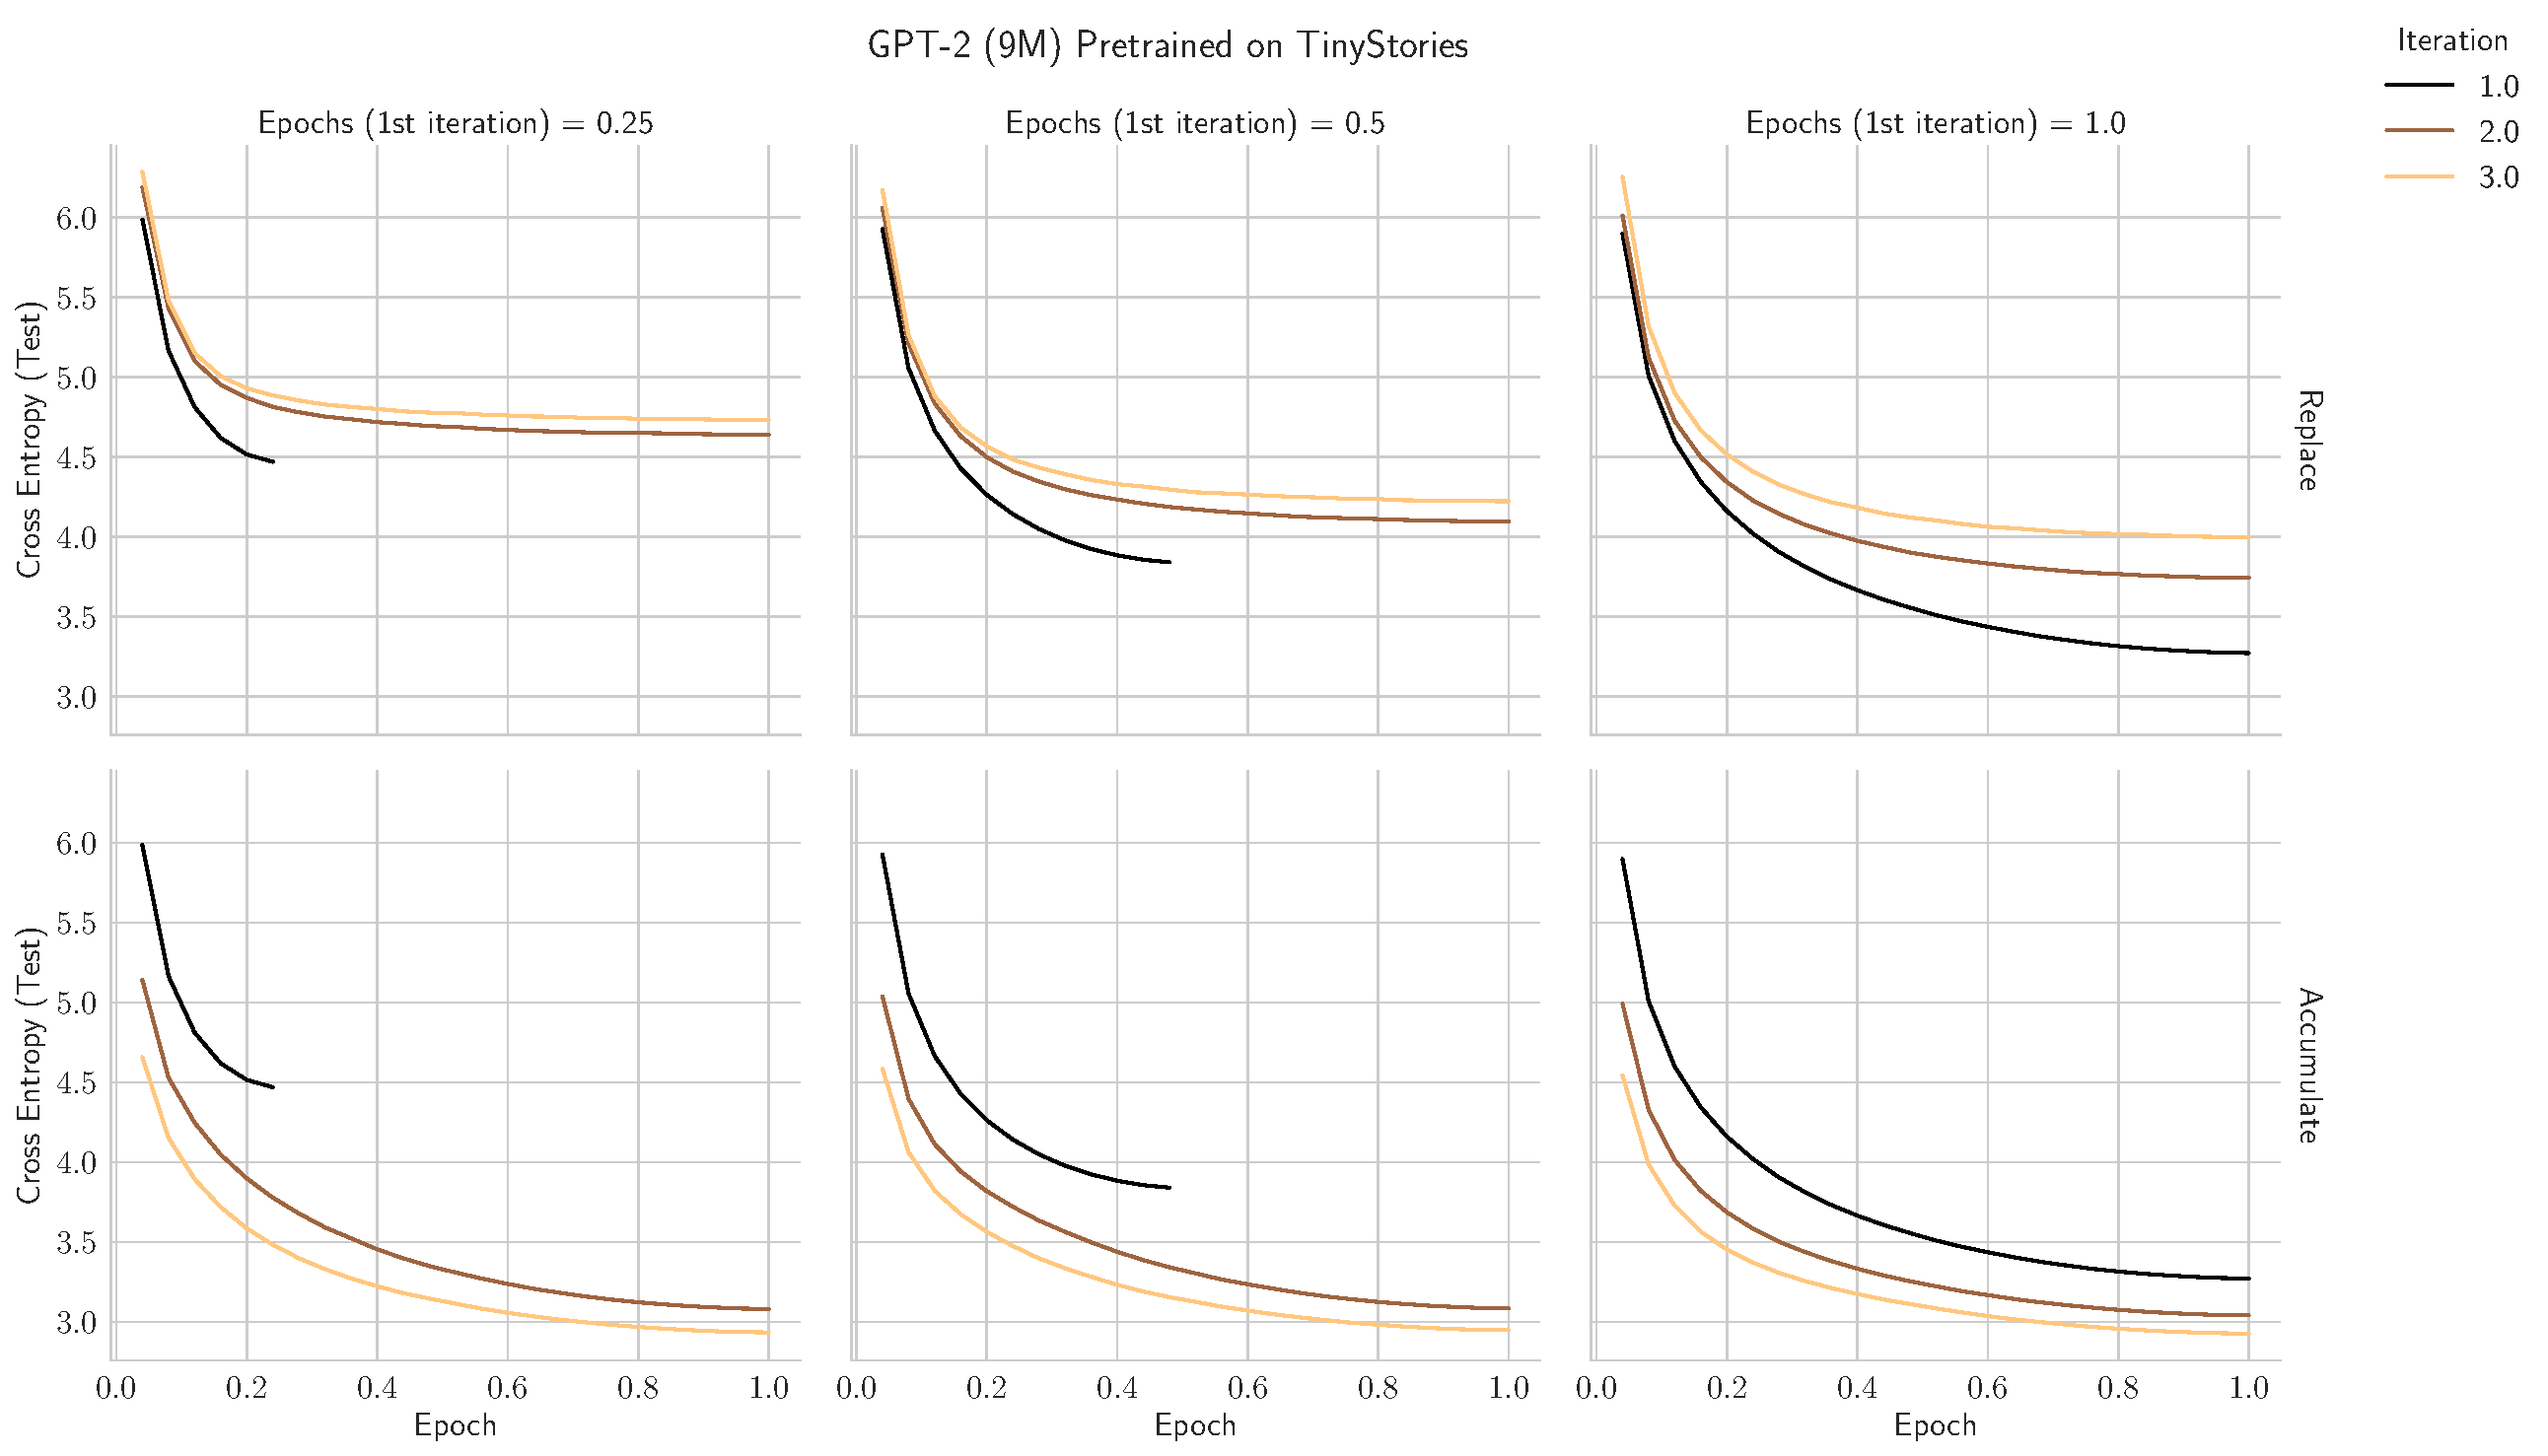
\includegraphics[width=\textwidth]{figures/language_modeling/eval_loss_vs_firstiter_20240329_220900.pdf}
    \caption{Model quality after the first model-fitting iteration does not qualitatively change behavior in subsequent iterations. Columns show differing training amount (as measure by epochs) in first iteration.
    }
    \label{fig:language_modeling_firstiter}
\end{figure}




\clearpage
\section{Additional Details on VAE Experiments}
\label{app:sec:vae_ablations}
\paragraph{Experiment Details.}
As pre-processing, we crop and down-sample the images to 64x64 pixels. We use a standard convolutional architecture for the VAE model consisting of 5 convolutional layers with 32, 64, 128, 256, and 512 channels, respectively, and a similar convolutional decoder structure. The latent space is 128-dimensional isotropic Gaussian, represented by 2 MLP layers. Each data iteration consists of 100 training epochs, after which we generate 163K new training images by sampling latents from the Gaussian prior and the passing them through the generator model.

\paragraph{Analysis of Reconstructions.}
Figure~\ref{fig:vae_reconstructions} shows reconstructions after replacing (left) and accumulating (center) data, compared to baseline (right).
Analyzing the reconstruction of test set images also reveals interesting findings - the model trained only on data from the prior iteration has indeed collapsed and cannot represent any other classes besides the single mode it generates. Interestingly, the model trained on aggregated data still maintains it's capabilities and generates accurate reconstructions, including smaller details such as glasses and hats. We hypothesize that this model maintains it's generative capabilities, but these details become a more minor sub-manifold in the latent space, which is realigned with the newly-generated data, hence why they appear less often in the generated images, which use samples from the prior.


\begin{figure}[h!]
    \centering
    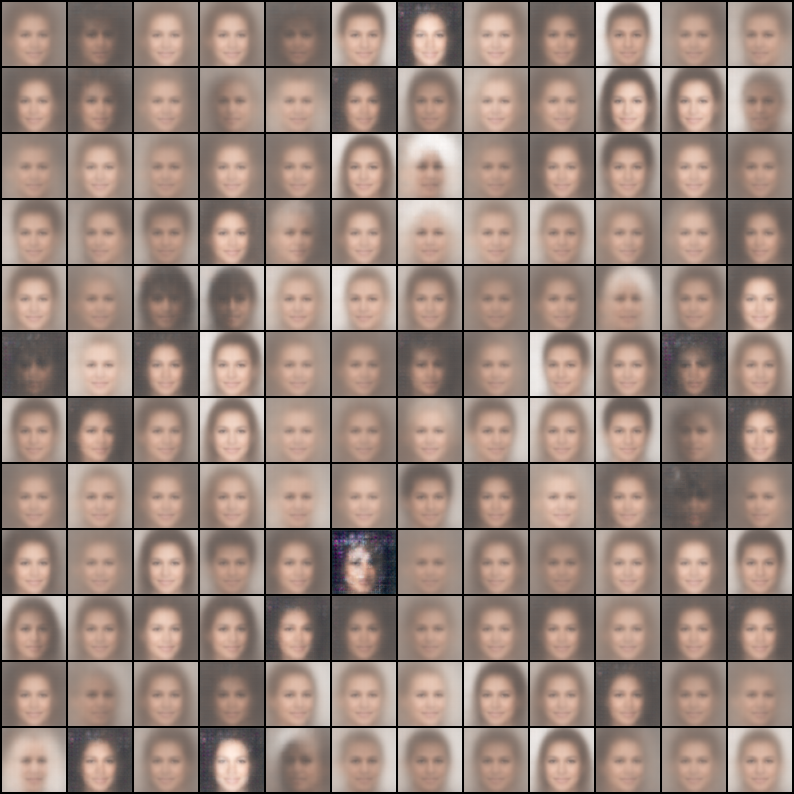
\includegraphics[width=0.325\textwidth]{figures/image_vae/no_aggregate_recon.png}
    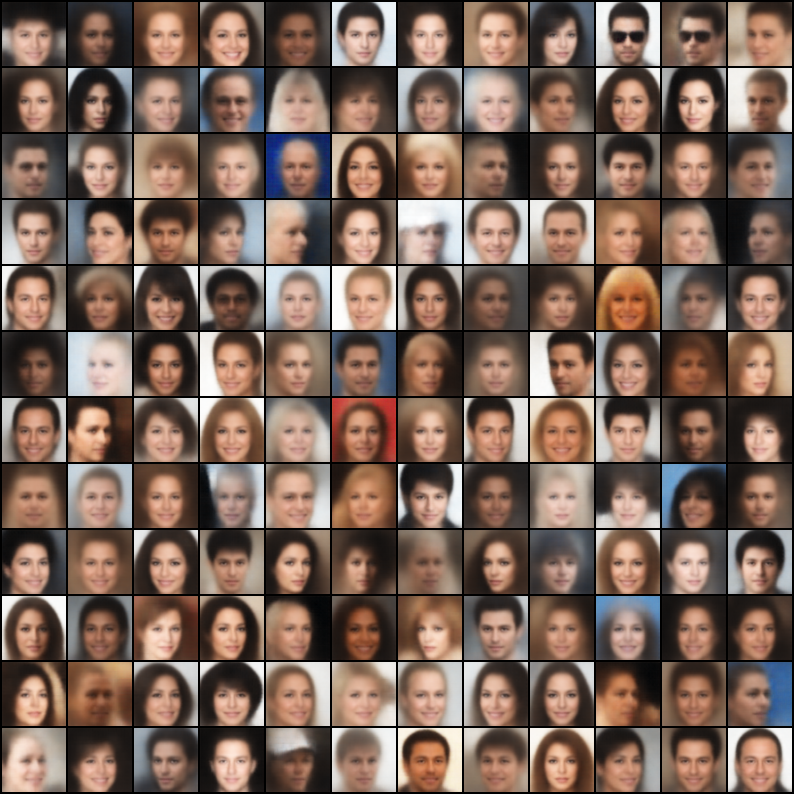
\includegraphics[width=0.325\textwidth]{figures/image_vae/aggregate-recon.png}
    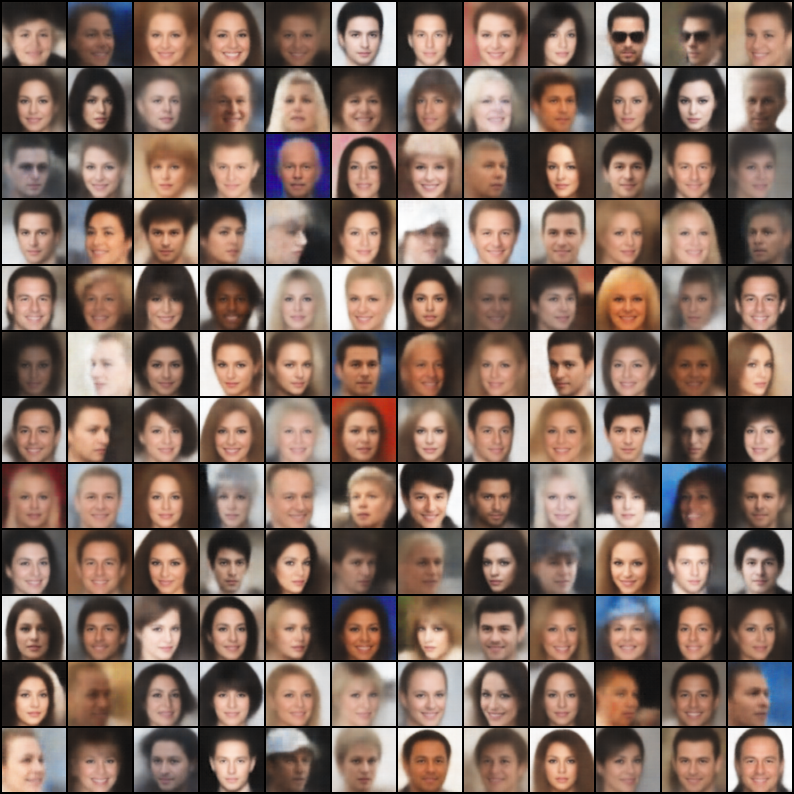
\includegraphics[width=0.325\textwidth]{figures/image_vae/continual_recon.png}

    
    \caption{\textbf{Data Accumulation Maintains Model Capabilities.} Image reconstructions from the test set. Left: Training on prior iterations collapses the model's capability, and subsequently, it can only represent a single mode. Middle: training on aggregated data preserves model capabilities and leads to little to no degradation in the reconstructed images. Right: Baseline reconstructions after 100 training epochs on the dataset.}
    \label{fig:vae_reconstructions}
\end{figure}





























\clearpage
\section{Linear Regression: Replacing Data with Increasing Sample Size}
\label{app:sec:linear_reg_replace_multiple}

In the framework of \citet{mobahi2020self} and \citet{dohmatob2024model}, we consider sequences of linear models fit to the previous model's synthetic outputs. Within this framework, \citet{dohmatob2024model} proved that \replace{if data are replaced} with each model fitting iteration and the training data cardinality remains constant, \replace{then the test squared error scales linearly with the number of model fitting iterations $n$}:

\begin{equation}
E_{\text{test}}^{\text{Replace}}(\hat{w}_n) = \frac{\sigma^2 d}{T - d -1} \times \color{red}n \color{black}
\end{equation}

In this work, we lightly adapt the argument of \citet{dohmatob2024model} to study the effects \accumulate{if data accumulate} with each model fitting iteration. We specifically considered the case where the training data cardinality increases by a constant $T$ with each model-fitting iteration i.e. the $i$th model is fit using $T\times i$ data, where $T$ data are ``real" and then each subsequently fit model contributes its own $T$ synthetic data to the accumulating data. In this setting, \accumulate{the test squared error is upper bounded independent of the number of iterations}.

\begin{equation}
E_{\text{test}}^{\text{Accumulate}}(\hat{w}_n) = \frac{\sigma^2 d}{T - d -1} \times \sum_{k=1}^n \dfrac{1}{k^2} \leq \frac{\sigma^2 d}{T - d -1} \times \color{red}\frac{\pi^2}{6} \color{black}
\end{equation}

In the main text, we focus on the replace and accumulate data settings because prior work focused on replacing data and we wished to study how accumulating data affects model collapse. However, a much richer landscape of outcomes is possible. For instance, and as pointed out in personal correspondence with \citet{dohmatob2024model}, one can consider what we term the \replacemultiple{``Replace-Multiple"} setting, in which one fits the $i$-th linear model using $T\times i$ data sampled from the $(i-1)$-th linear model. Replace-Multiple is a useful baseline for Accumulate because it matches the amount of training data at each model fitting iteration. Under \replacemultiple{Replace-Multiple, the test squared error grows logarithmically}:

\begin{equation}
E_{\text{test}}^{\text{Replace-Multiple}}(\hat{w}_n) = \frac{\sigma^2 d}{T - d -1} \times \sum_{k=1}^n \dfrac{1}{k} \approx \frac{\sigma^2 d}{T - d -1} \times \color{red} \log(n) \color{black}
\end{equation}

Replace-Multiple has the drawback of not matching the total amount of compute of Accumulate since each iteration of Replace-Multiple draws $T\times i$ samples from the most recent model, whereas Accumulate draws $T$ samples from the most recent model. 
Other baselines are also possible, but we leave these to future work. We focus on accumulating data as we feel real and synthetic data are likely to accumulate in the real world as time progresses.

\clearpage
\section{Additional Linear Regression Numerical Results}
\label{app:sec:linear_regression_numerics}

\begin{figure}[h!]
    \centering
    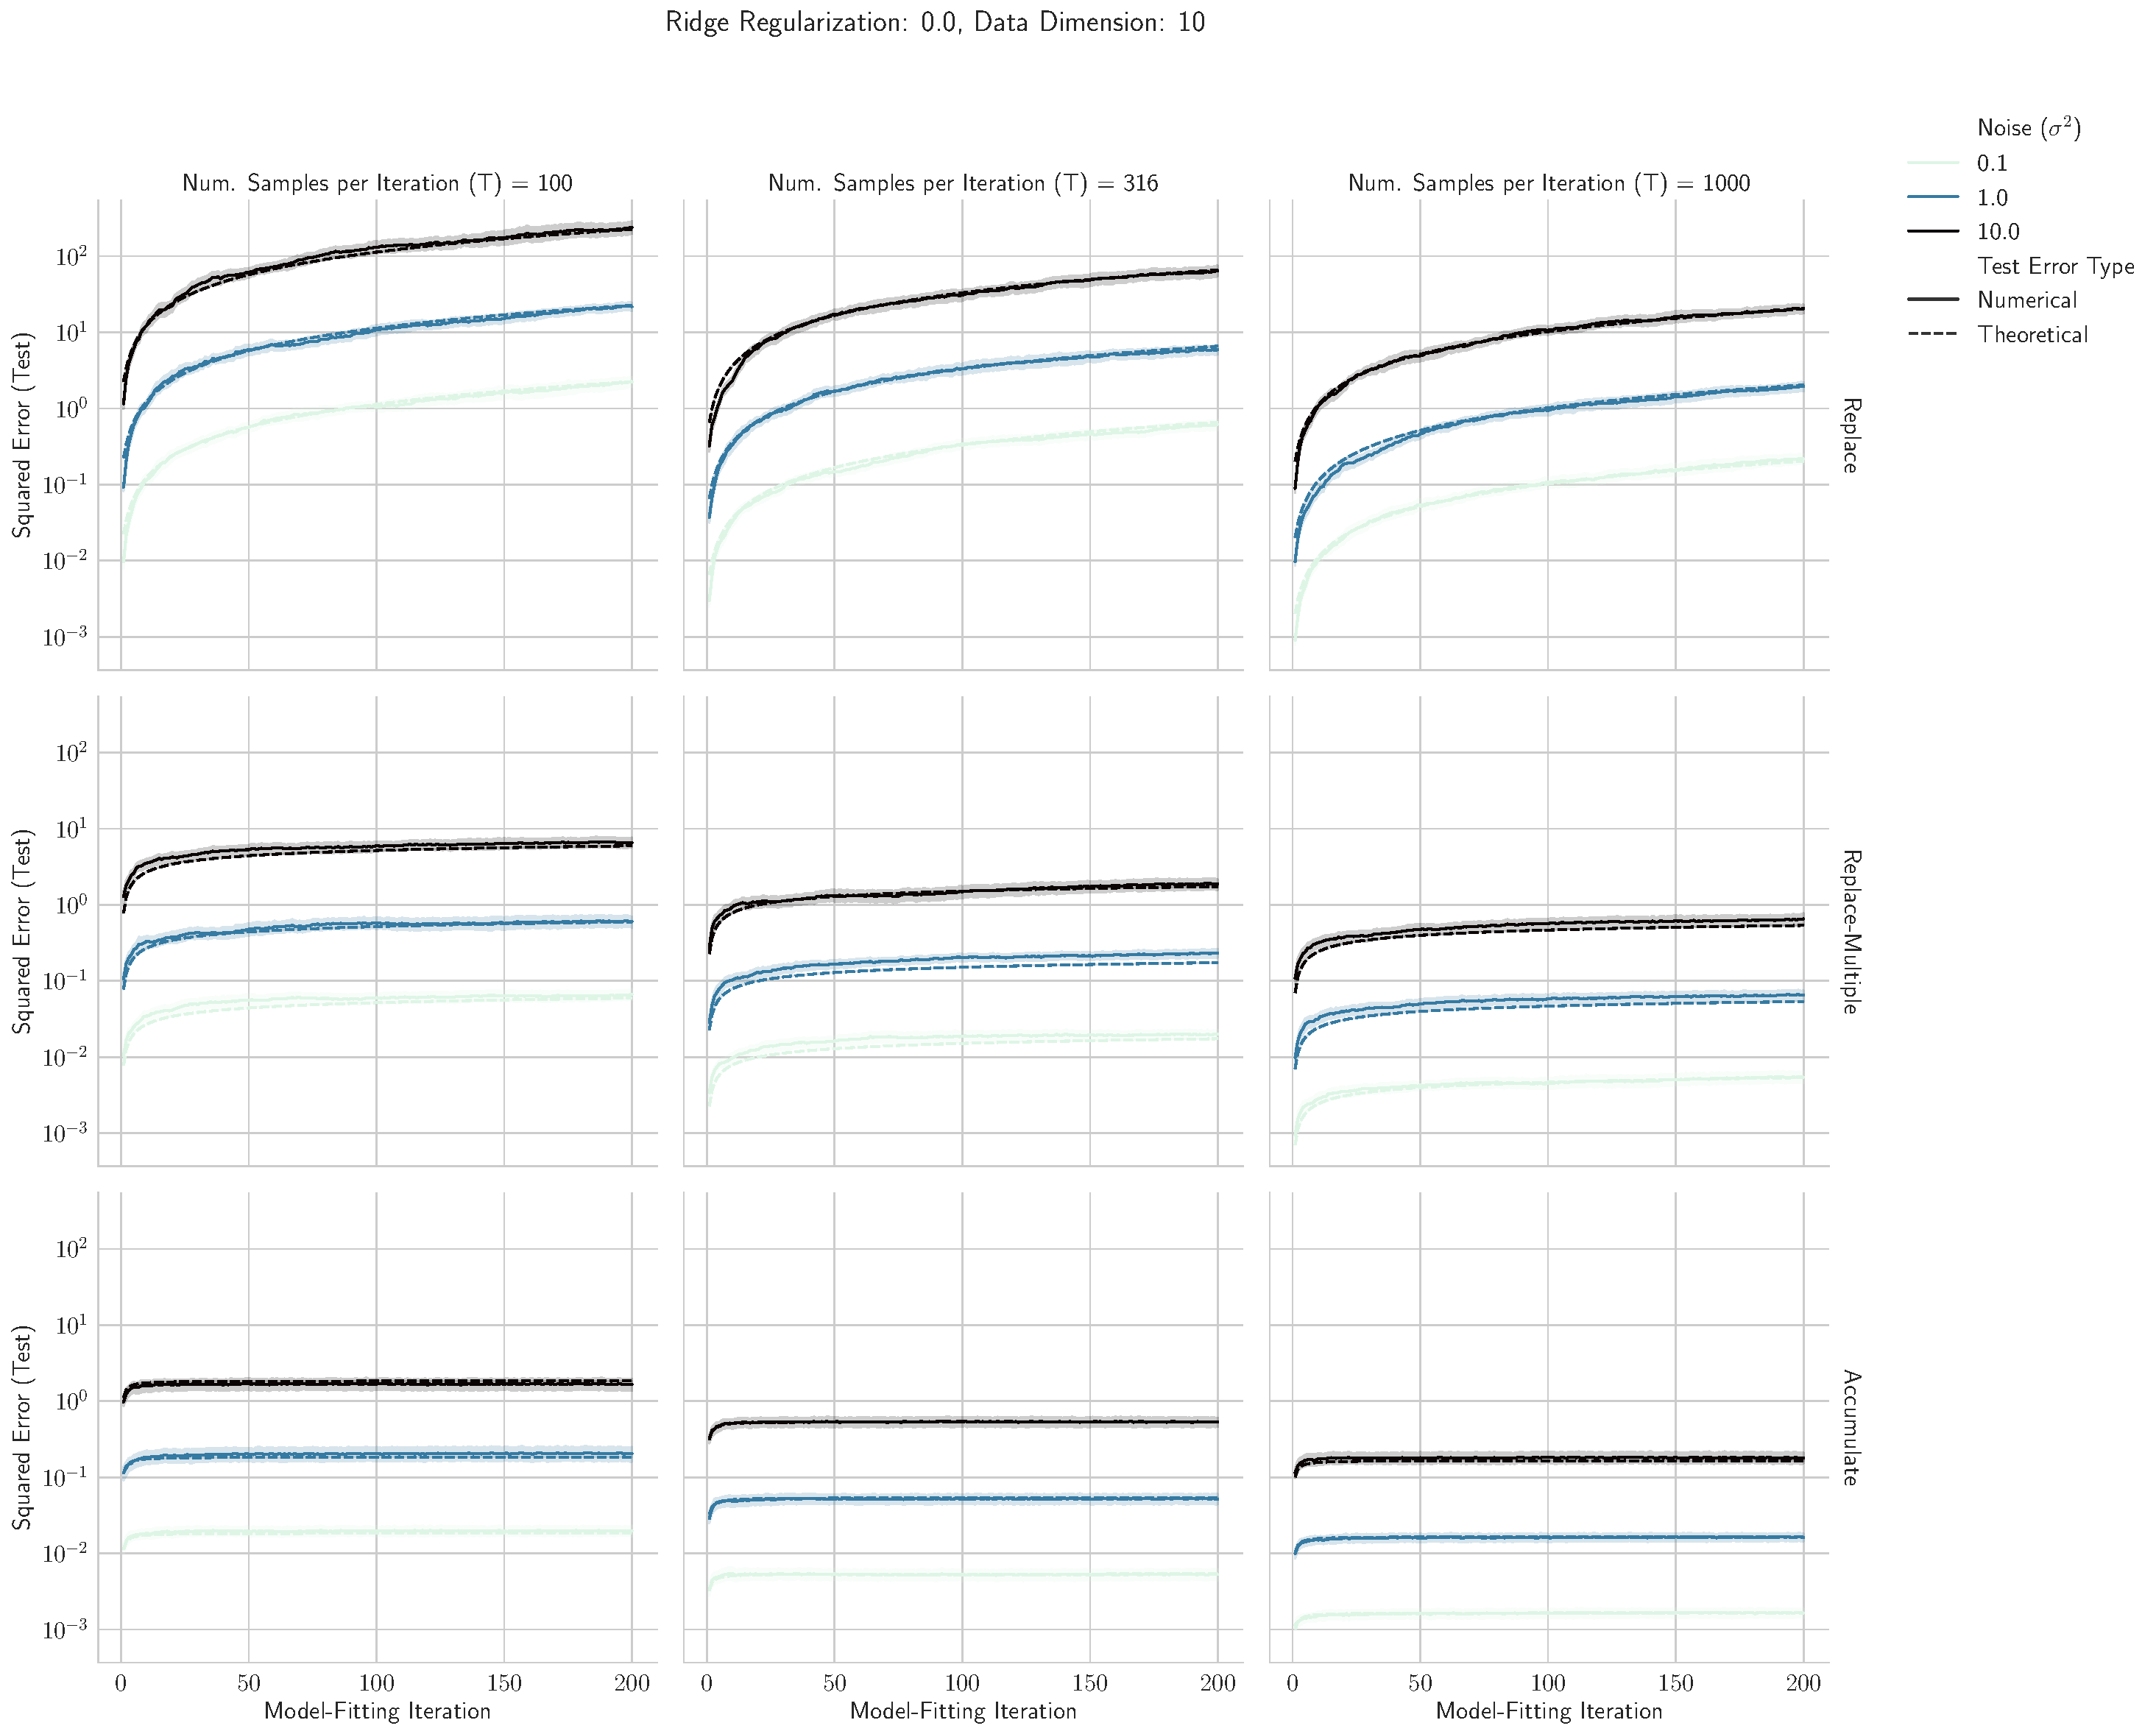
\includegraphics[width=\textwidth]{figures/linear_regression/isotropic_features_log_linear_lambda=0.0_d=10.pdf}
    \caption{\textbf{Accumulating data across iterations avoids model collapse in linear regression.} We consider sequences of linear models recurrently fit to generated targets by previous iterations of models. \replace{Replace} (Top): If each linear model is fit to the generated targets of \textit{only} the preceding linear model i.e. data are replaced, then the \replace{test squared error grows linearly} with the number of model-fitting iterations iterations $n$. \replacemultiple{Replace-Multiple} (Middle): If each linear model is fit to $T\times i$ samples from the $(i-1)$-th model (i.e. the same amount of data as Accumulate), then the \replacemultiple{test squared error grows logarithmically} with the number of model-fitting iterations; see Appendix \ref{app:sec:linear_reg_replace_multiple} for more details. \accumulate{Accumulate} (Bottom): If each linear model is instead fit to the generate targets of \textit{all} the preceding linear models i.e. data accumulate, then the \accumulate{test squared error has a finite upper bound, independent of the number of iterations}. 
    This suggests that data accumulation might be a robust solution for mitigating model collapse. This figure is similar to Figure \ref{fig:accumulating_vs_nonaccumulating_isotropic_features} but displaying \textit{log} test squared error and more model-fitting iterations for additional clarity.}
    \label{app:fig:accumulating_vs_nonaccumulating_isotropic_features_log_linear}
\end{figure}



\newpage

